% ============================================================
%  Chapter 11 — Dynamic Vehicle Routing Problems
%  Source: Vehicle Routing: Problems, Methods, and Applications
%          2nd edition, 2014.  Chapter by Bektas, Repoussis,
%          and Tarantilis.
%  Self-contained Beamer slides (reader-friendly, no presenter).
% ============================================================
\documentclass[aspectratio=169,10pt]{beamer}

\usetheme{Madrid}
\usecolortheme{seahorse}
\setbeamertemplate{footline}[frame number]
\setbeamertemplate{navigation symbols}{}

% ── Packages ─────────────────────────────────────────────────
\usepackage{amsmath,amssymb,amsthm}
\usepackage{graphicx}
\usepackage{booktabs}
\usepackage{array}
\usepackage{xcolor}
\usepackage{listings}
\usepackage{microtype}
\usepackage{tikz}
\usetikzlibrary{shapes.geometric,arrows.meta,positioning,fit}
\usepackage{hyperref}

\graphicspath{{figures/}}

% ── Listings style ───────────────────────────────────────────
\lstset{
  language=Python,
  basicstyle=\ttfamily\scriptsize,
  numbers=left,
  numberstyle=\tiny\color{gray},
  frame=single,
  backgroundcolor=\color{gray!7},
  commentstyle=\color{green!50!black}\itshape,
  keywordstyle=\color{blue!70!black}\bfseries,
  stringstyle=\color{orange!80!black},
  breaklines=true,
  showstringspaces=false,
  tabsize=4,
}

% ── Title slide info ─────────────────────────────────────────
\title[Dynamic VRP]{Chapter 11: Dynamic Vehicle Routing Problems}
\subtitle{Vehicle Routing: Problems, Methods, and Applications\\
          2nd Edition, 2014}
\author{Tolga Bektas \and Panagiotis P. Repoussis \and Christos D. Tarantilis}
\date{Slides prepared for self-study}
\institute[VRP Lectures]{Vehicle Routing Lecture Series}

% ─────────────────────────────────────────────────────────────
\begin{document}
% ─────────────────────────────────────────────────────────────

\begin{frame}
  \titlepage
\end{frame}

% ────────────────────────────────────────────────────────────
\begin{frame}{Table of Contents}
  \tableofcontents
\end{frame}

% ============================================================
\section{Introduction}
% ============================================================

\begin{frame}[allowframebreaks]{Introduction — Why Routing is Never Truly Static}

  Real-world vehicle routing is rarely a ``plan-once, execute-perfectly'' problem.
  In most operational settings, the values of all input parameters are not known
  with certainty at the moment the planning horizon begins.
  Instead, information arrives \emph{gradually} during the day: new customer
  requests are called in by phone or submitted via a mobile app, traffic jams
  develop unexpectedly, or a vehicle breaks down and must be taken out of service.

  A classical, static Vehicle Routing Problem (VRP) assumes that all information
  is known \emph{in advance} and \emph{with certainty} before any vehicle leaves
  the depot.  That assumption is violated in practice in at least three important
  ways:
  \begin{itemize}
    \item \textbf{Dynamic requests.}  New customers may call during the day,
          requiring the dispatcher to insert them into already-running routes.
    \item \textbf{Dynamic travel times.}  Congestion, road closures, and weather
          make travel times depend on the time of day and change unpredictably.
    \item \textbf{Dynamic vehicle availability.}  Vehicles break down, become
          unavailable within certain windows, or return late from previous tours.
  \end{itemize}

  The field of \textbf{Dynamic Vehicle Routing} (DVR) addresses all three of these
  complications.  The goal is to develop routing and dispatching algorithms that
  respond in real time to a changing environment whilst still producing
  high-quality, operationally feasible plans.

  \framebreak

  \begin{block}{Why dynamic routing is harder than static routing}
    In a static VRP, the algorithm has unlimited time to compute an optimal plan
    because all data are fixed before execution begins.  In a dynamic setting,
    the algorithm must (i)~react to new information within seconds (because a
    waiting vehicle or a waiting customer is expensive), (ii)~decide which
    actions to commit to \emph{now} versus which to defer, and (iii)~balance
    the quality of the current plan against the anticipated quality of plans
    that will be needed after future, as-yet-unknown events.
  \end{block}

  \begin{alertblock}{Key insight}
    The difficulty of dynamic VRP is not purely computational — it is also
    \emph{informational}.  The algorithm must reason about what it does not
    yet know and act under genuine uncertainty about the future.
  \end{alertblock}

  Advances in technology have made dynamic routing increasingly tractable.
  GPS devices provide real-time vehicle positions; mobile and radio networks
  relay customer requests instantly; on-board computers accept re-routing
  instructions while vehicles are moving.  These technologies have made
  dynamic dispatching systems commercially feasible and have stimulated a
  growing research literature.

  \begin{figure}
    \centering
    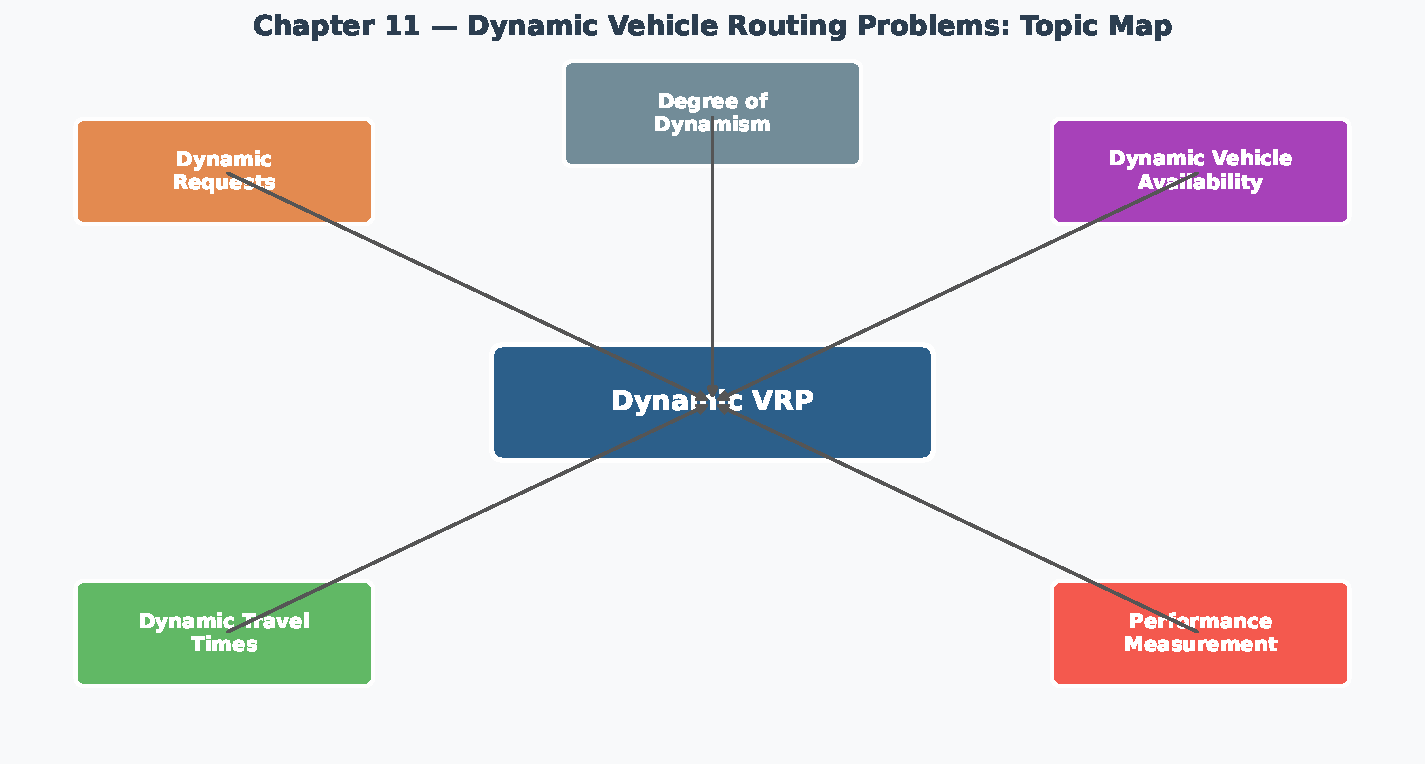
\includegraphics[width=0.85\textwidth]{ch11_overview.pdf}
    \caption{Topic map of Chapter~11.  The chapter covers three main sources of
             dynamism (requests, travel times, vehicle availability) and discusses
             how to measure solution quality under uncertainty.}
  \end{figure}

\end{frame}

% ============================================================
\section{Definitions, Objectives, and Problem Variants}
% ============================================================

\begin{frame}[allowframebreaks]{The Dynamic VRP — Formal Definition}

  The chapter builds on the definition provided by Psaraftis~(1995) and extends
  it to capture the modern operational landscape.

  \begin{block}{Definition: Dynamic VRP}
    A \textbf{Dynamic Vehicle Routing Problem} is a VRP in which some or all
    input parameters are not known at the beginning of the planning horizon
    but are \emph{revealed progressively} while vehicles are executing their
    routes.  The dispatcher must update the plan each time new information
    arrives, subject to operational constraints.
  \end{block}

  In mathematical terms, let time be indexed by $t \in [0, T]$ where $T$ is
  the end of the planning horizon.  At $t = 0$, a set of \emph{a priori} (that
  is, known-in-advance) customers $C^0$ is available.  During the horizon,
  additional customers $C^t$ may arrive at random times $t > 0$.
  The full customer set at any time $t$ is therefore $C^0 \cup C^t$.
  The dispatcher must assign all customers in $C^0 \cup C^T$ to vehicle routes
  whilst updating route assignments continuously as new customers arrive.

  \framebreak

  \begin{block}{Key terminology}
    \begin{description}
      \item[A priori customers:] Requests that are known before the planning
        horizon begins; they can be included in an initial route plan.
      \item[Dynamic customers:] Requests that arrive after the horizon begins;
        they must be inserted into existing routes in real time.
      \item[Committed actions:] Actions that have already been \emph{executed}
        by a vehicle and cannot be undone — for example, a delivery already
        made or a visit already begun.
      \item[Planned actions:] Actions assigned to a vehicle in the current plan
        but not yet begun; these \emph{can} be revised when new information arrives.
    \end{description}
  \end{block}

  The distinction between committed and planned actions is central to dynamic
  routing: the dispatcher has freedom to re-plan future stops, but must not
  override stops that are already in progress.

  \framebreak

  \begin{figure}
    \centering
    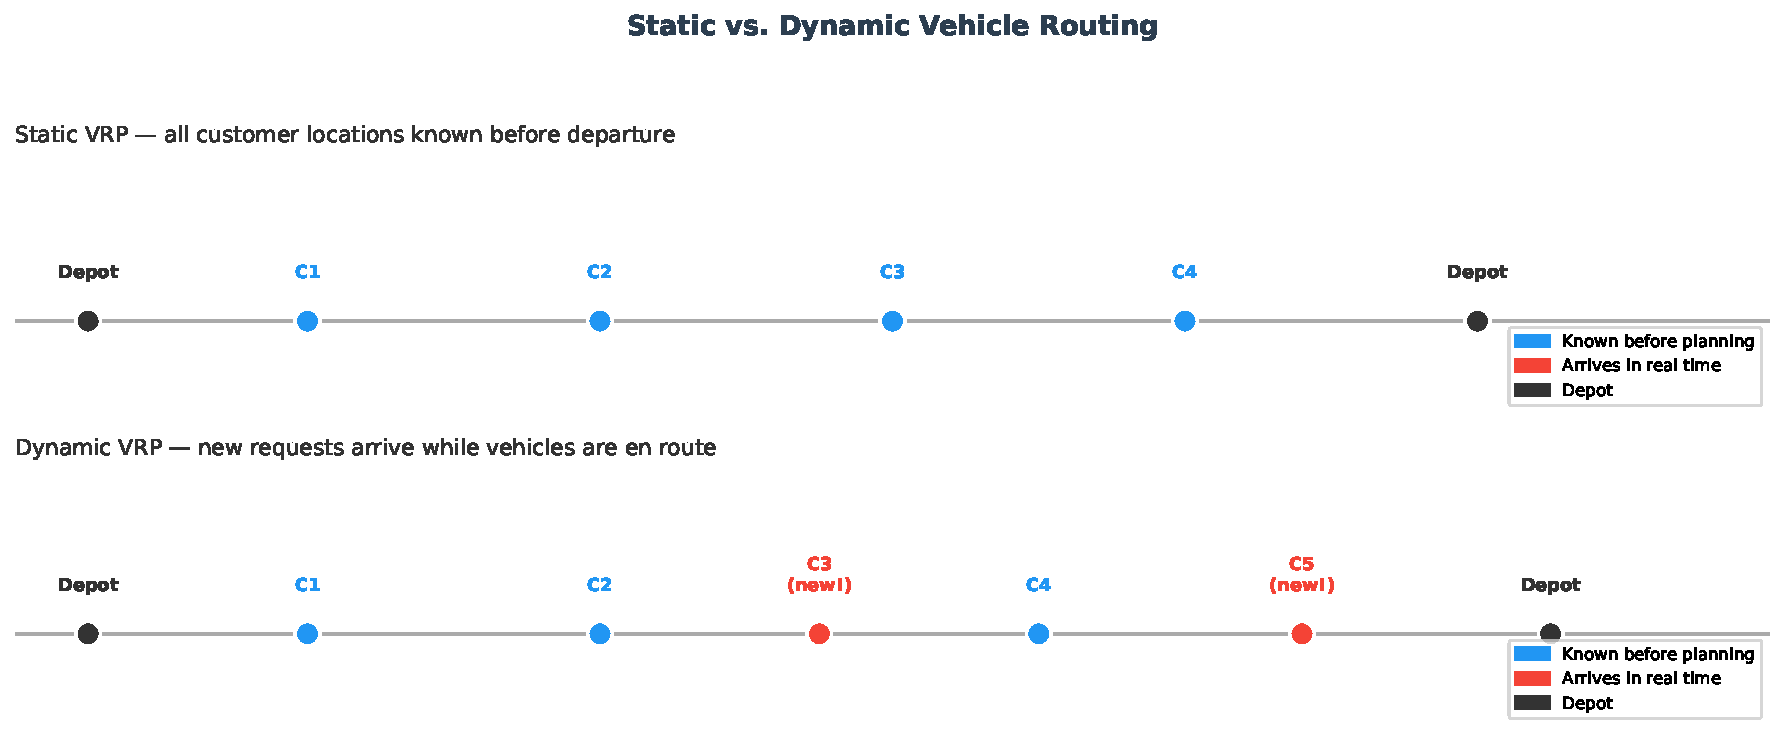
\includegraphics[width=0.88\textwidth]{ch11_static_vs_dynamic.pdf}
    \caption{In a static VRP (top), all customer locations are fixed before any
             vehicle moves.  In a dynamic VRP (bottom), new requests (red
             triangles) arrive while vehicles are already on the road, forcing
             real-time re-planning.}
  \end{figure}

\end{frame}

% ────────────────────────────────────────────────────────────
\begin{frame}[allowframebreaks]{Sources of Dynamism — Three Categories}

  The chapter identifies three distinct sources of dynamism that arise in
  real-world vehicle routing:

  \medskip
  \textbf{1. Dynamic requests} (Section~11.3 of the book).
  New customer service requests arrive during the planning horizon.
  A taxi dispatching system, a same-day parcel delivery service, or an
  emergency ambulance system all face this type of dynamism.
  The key challenge is to insert each new request into the current set of
  routes while disrupting existing commitments as little as possible.

  \medskip
  \textbf{2. Dynamic and time-dependent travel times} (Section~11.4 of the book).
  Travel times between locations change throughout the day due to congestion,
  traffic signals, road closures, and weather.  This affects both route
  planning (which roads to take) and scheduling (when to arrive at each stop).

  \medskip
  \textbf{3. Dynamic vehicle availability} (Section~11.5 of the book).
  Vehicles may break down, may only become available after a certain time,
  or may need servicing mid-day.  When a vehicle breaks down, its remaining
  customers must be redistributed to other vehicles, potentially requiring
  complete re-optimisation.

\end{frame}

% ────────────────────────────────────────────────────────────
\begin{frame}[allowframebreaks]{Degree of Dynamism}

  Not all dynamic VRP instances are equally dynamic.  To compare algorithms
  fairly across problem types, researchers have proposed various measures of
  how \emph{dynamic} a problem instance is.  The most widely cited measure is
  the \textbf{degree of dynamism} (dod), introduced by Larsen, Madsen, and
  Salomon~(2002) and extended by subsequent authors.

  \begin{block}{Degree of Dynamism (dod) — Original Definition (Larsen 2002)}
    Let $n_d$ denote the number of \emph{dynamic} (online) customer requests
    that arrive after the planning horizon begins, and let $n$ denote the
    \emph{total} number of customers (both known and dynamic).
    The degree of dynamism is defined as:
    \[
      \mathrm{dod} = \frac{n_d}{n}
    \]
    where $n_d$ (read: ``n sub d'') is the count of dynamically arriving
    requests and $n$ is the total number of requests.
  \end{block}

  \begin{block}{Notation}
    Here $n_d$ counts only the customers whose locations were \emph{not} known
    when the initial plan was computed.  $n$ is the sum of all customers,
    both pre-known and dynamically arriving.
    The ratio $\mathrm{dod}$ (degree of dynamism) therefore falls in the
    interval $[0, 1]$: a value of $0$ means a fully static problem
    (all customers known in advance), while a value of $1$ means a fully
    dynamic problem (no customers known in advance at all).
  \end{block}

  \begin{alertblock}{How to read this formula}
    As $\mathrm{dod}$ increases, the problem becomes harder for \emph{anticipatory}
    algorithms (which plan ahead) and easier for purely reactive algorithms
    (which only respond to what is already known).  At very high dod values,
    there is little advance information to exploit, so sophisticated
    look-ahead strategies provide diminishing returns.
  \end{alertblock}

  \framebreak

  \begin{block}{Effective Degree of Dynamism (Larsen 2002, extended)}
    A criticism of the simple dod measure is that it ignores \emph{when}
    dynamic requests arrive.  A request arriving at the very start of the
    horizon is almost as useful as a known request, whereas a request arriving
    in the last few minutes is extremely disruptive.
    The \textbf{effective degree of dynamism} ($\mathrm{edod}$) accounts for
    this by weighting each dynamic request by how late in the horizon it arrives:
    \[
      \mathrm{edod} = \frac{1}{n} \sum_{i=1}^{n_d} \frac{t_i^{\mathrm{arrive}}}{T}
    \]
    where $t_i^{\mathrm{arrive}}$ (read: ``t sub i superscript arrive'') is the
    time at which dynamic request $i$ becomes known, and $T$ is the total
    length of the planning horizon.
  \end{block}

  \begin{block}{Notation for edod}
    The sum runs over all $n_d$ dynamic requests.  The fraction
    $t_i^{\mathrm{arrive}} / T$ is a number between $0$ and $1$: it equals
    $0$ if the request arrives at the very beginning and $1$ if it arrives
    at the very end.  Dividing the entire sum by $n$ (total customers)
    normalises the metric so that it also lies in $[0, 1]$.
  \end{block}

  \begin{alertblock}{Intuition}
    The edod formula says: ``on average, how late in the planning day do the
    dynamic requests arrive?''  A high edod means most surprises come late,
    leaving less time to re-route, which makes the problem harder.
  \end{alertblock}

  \framebreak

  \begin{figure}
    \centering
    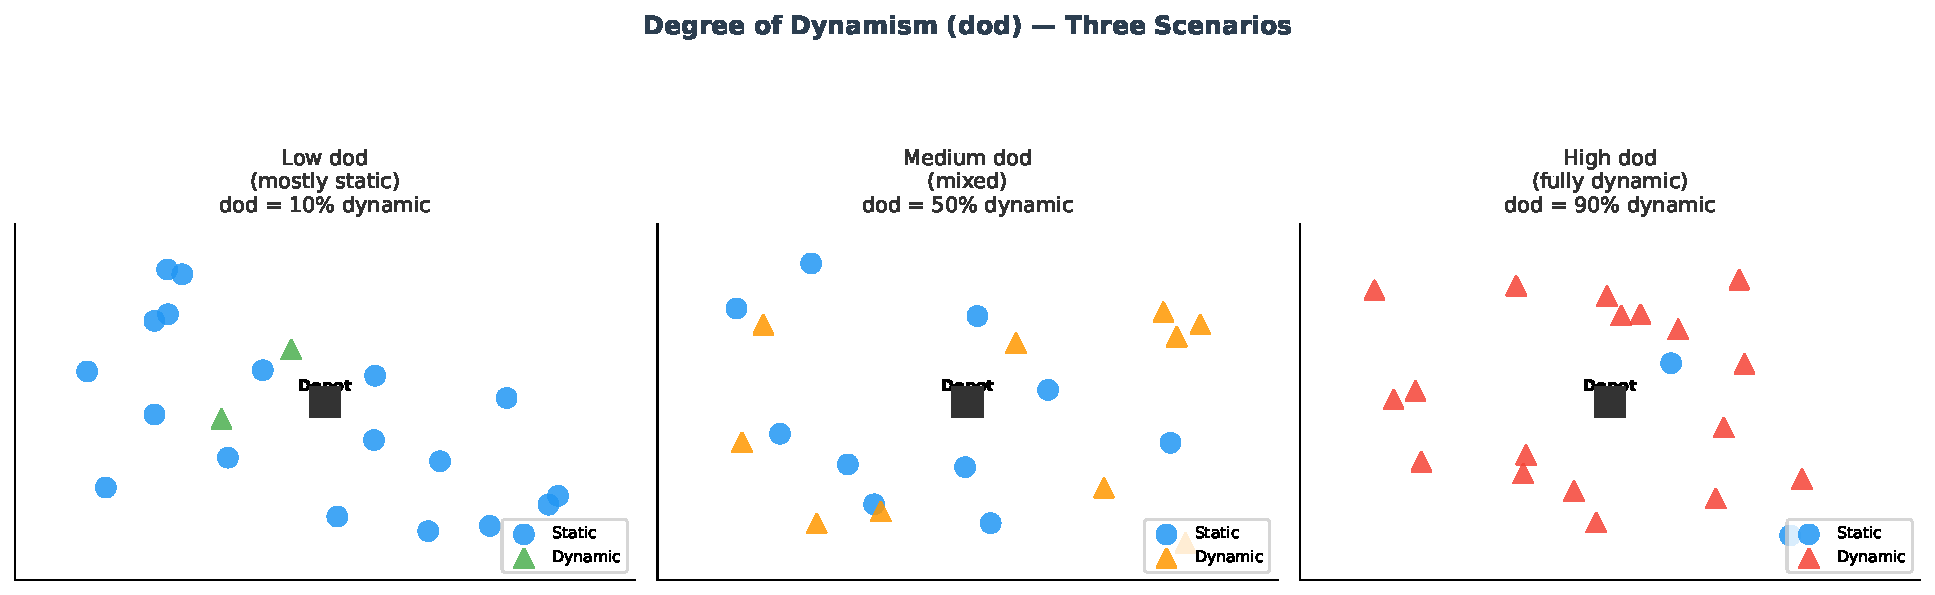
\includegraphics[width=0.85\textwidth]{ch11_degree_of_dynamism.pdf}
    \caption{Illustration of the degree of dynamism across three problem instances.
             Blue circles are customers known before planning starts; coloured
             triangles are customers that arrive dynamically.
             Low dod (left) means most customers are known in advance.
             High dod (right) means most customers arrive in real time.}
  \end{figure}

  \framebreak

  \begin{block}{Objectives in Dynamic VRP}
    The primary objective in most dynamic VRP formulations is to minimise
    total travel distance (or total travel time) over all vehicles:
    \[
      \text{Minimise} \quad Z = \sum_{k=1}^{K} \sum_{(i,j) \in A} d_{ij} \, x_{ijk}
    \]
    where $K$ is the number of vehicles, $A$ is the set of arcs (directed road
    segments between customer locations and the depot), $d_{ij}$ (d sub i j) is
    the travel distance from node $i$ to node $j$, and $x_{ijk}$ (x sub i j k)
    is a binary decision variable equal to $1$ if vehicle $k$ travels directly
    from node $i$ to node $j$ on its route, and $0$ otherwise.
  \end{block}

  \begin{block}{Notation}
    $K$ = number of vehicles in the fleet; $A$ = set of all arcs (ordered
    pairs of locations); $d_{ij}$ = distance (or time) from location $i$ to
    location $j$; $x_{ijk} \in \{0, 1\}$ = 1 if vehicle $k$ uses arc $(i,j)$.
  \end{block}

  Other commonly used objectives include minimising the number of vehicles
  used, minimising the number of rejected (unserved) dynamic requests, and
  minimising waiting times for customers.  A \textbf{hierarchical objective}
  may first minimise the number of vehicles and then minimise total distance.

\end{frame}

% ────────────────────────────────────────────────────────────
\begin{frame}[allowframebreaks]{Problem Variants — Taxonomy}

  The chapter distinguishes between several broad categories of dynamic VRP:

  \medskip
  \textbf{Static and deterministic.}  All parameters are known and fixed.
  This is the classical VRP; it provides the benchmark against which dynamic
  approaches are compared.

  \medskip
  \textbf{Static and stochastic.}  All parameters are revealed before execution
  begins, but some of them (such as customer demand) are random variables.
  The algorithm plans once using probabilistic information.

  \medskip
  \textbf{Dynamic and deterministic.}  Parameters are revealed over time, but
  once revealed they are exact (no noise or uncertainty).  For example, a new
  customer request arrives at time $t$ with a precisely known location and demand.

  \medskip
  \textbf{Dynamic and stochastic.}  The most general case: parameters are revealed
  over time \emph{and} involve uncertainty.  For example, a customer may request
  service but their exact demand is only known upon vehicle arrival.  Emergency
  medical dispatch systems often fall into this category.

  \framebreak

  \begin{block}{The focus of this chapter}
    The chapter concentrates on \textbf{dynamic and deterministic} problems
    because this is where the largest body of literature exists and where the
    distinction between reactive versus anticipatory approaches is clearest.
    Stochastic aspects are mentioned where relevant, particularly in discussions
    of anticipatory algorithms that use probabilistic models of future arrivals.
  \end{block}

  \medskip
  Common specific problem types discussed include:
  \begin{itemize}
    \item \textbf{Dynamic VRPTW}: VRP with Time Windows where both requests
          and time windows may be dynamic.
    \item \textbf{Dynamic Dial-a-Ride} (DARP): pick-up and delivery of passengers,
          with dynamic pick-up requests and time-window constraints.
    \item \textbf{Dynamic PDP}: pick-up and delivery problems where goods must
          be picked up from one location and delivered to another.
    \item \textbf{Same-day delivery}: parcel delivery in which orders placed
          during the day must be delivered the same day.
  \end{itemize}

  \framebreak

  \begin{figure}
    \centering
    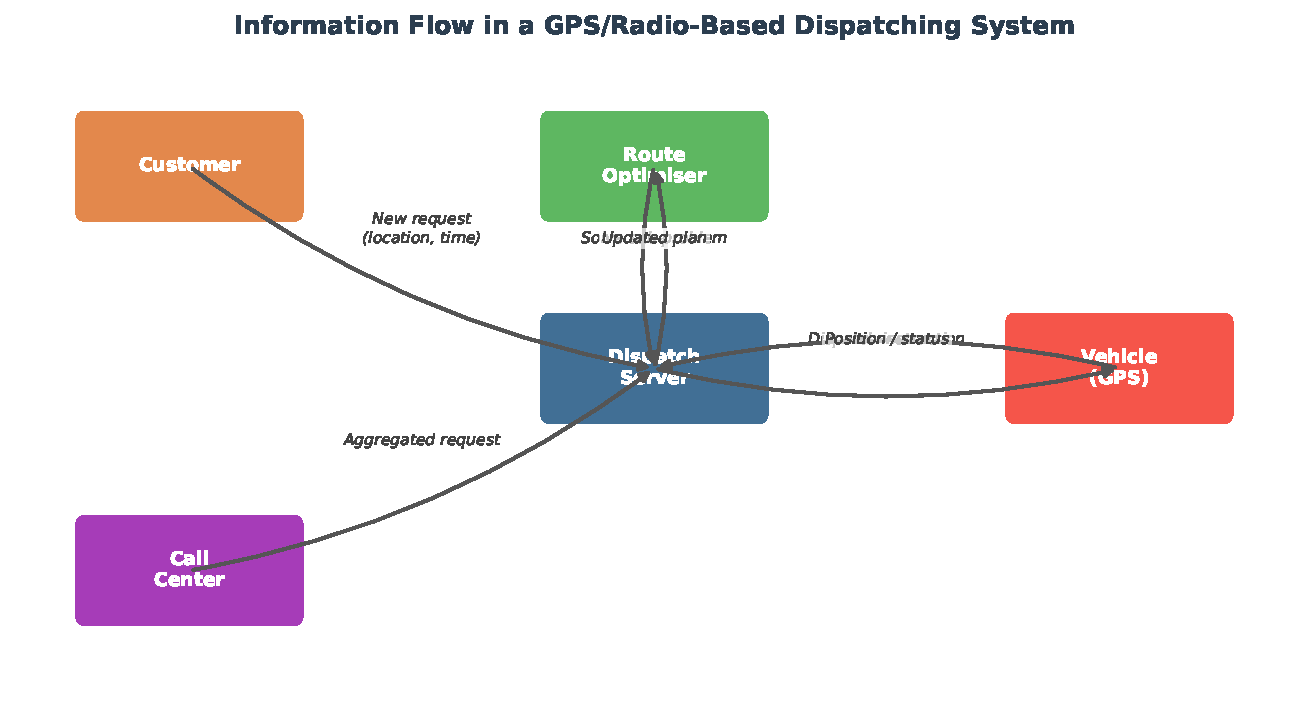
\includegraphics[width=0.90\textwidth]{ch11_information_flow.pdf}
    \caption{Information flow in a typical GPS-based dispatching system.
             Customers submit requests (upper left) or a call centre aggregates
             them; the dispatch server runs a route optimiser; and vehicles
             receive updated instructions via GPS/radio while transmitting
             their current positions back.  This loop typically runs every
             few minutes to seconds.}
  \end{figure}

\end{frame}

% ============================================================
\section{Dynamic Requests}
% ============================================================

\begin{frame}[allowframebreaks]{Dynamic Requests — The Core Challenge}

  The most studied form of dynamism in vehicle routing is the arrival of
  \emph{new service requests} during the execution of a plan.
  Consider a courier company whose drivers have already left the depot with
  a pre-planned schedule.  Throughout the day, new customers call in requesting
  delivery.  Each new request must be assigned to a vehicle and inserted into
  that vehicle's remaining route — ideally without requiring the vehicle to
  travel far out of its way.

  \begin{block}{Problem statement: Dynamic VRPTW with online requests}
    At time $t = 0$, a set $C^0$ of a priori customers is known and an initial
    route plan is computed.  During the planning horizon $[0, T]$, additional
    customers $c$ arrive one by one at times $t_c > 0$.  Each customer $c$ has:
    \begin{itemize}
      \item a location (coordinates or distance from other nodes);
      \item a service time $s_c$ (how long it takes to serve this customer);
      \item a time window $[e_c, l_c]$ where $e_c$ (e sub c) is the earliest
            acceptable service time and $l_c$ (l sub c) is the latest; and
      \item a demand $q_c$ (quantity to deliver or pick up).
    \end{itemize}
    The dispatcher must insert $c$ into a vehicle's route such that:
    (i) the vehicle's remaining capacity is not exceeded;
    (ii) all time windows (including those of already-scheduled customers)
         remain feasible; and (iii) the increase in total route cost is minimised.
  \end{block}

\end{frame}

% ────────────────────────────────────────────────────────────
\begin{frame}[allowframebreaks]{11.3.1 Dynamic vs. Deterministic Problems — Solution Strategies}

  The chapter classifies solution approaches for dynamic requests into three
  broad families: \textbf{reactive}, \textbf{periodic (rolling horizon)}, and
  \textbf{anticipatory} methods.  Each family represents a different attitude
  towards the future.

  \bigskip
  \textbf{Reactive methods} treat each new request independently and insert it
  into the current best route immediately when it arrives.  They make no
  attempt to reason about what future requests might look like.  Reactive
  methods are very fast and simple to implement, making them popular in
  practice, but they can perform poorly when there are many future requests
  that could have been served more efficiently if the vehicle had been
  positioned differently.

  \bigskip
  \textbf{Periodic (rolling horizon) methods} re-optimise the complete route
  plan at regular time intervals — for example, every 5 minutes — rather than
  reacting to each individual request.  This allows several new requests to
  be consolidated into a single re-planning step, which often produces better
  routes than inserting them one at a time.

  \bigskip
  \textbf{Anticipatory methods} explicitly model the uncertainty about future
  requests and use that model to make better decisions today.  For example,
  rather than dispatching a vehicle immediately to a known customer, an
  anticipatory method might hold the vehicle at a good waiting position for a
  short time in case a cluster of new requests arrives nearby.

  \framebreak

  \begin{block}{Comparison of the three strategy families}
    \begin{tabular}{lllp{4.5cm}}
      \toprule
      Strategy & Reaction & Computation & Best suited for\\
      \midrule
      Reactive & Per event & Very fast & High dod, time-critical\\
      Periodic  & Every $\Delta t$ & Moderate & Mixed dod\\
      Anticipatory & Per event + look-ahead & Expensive & Low-medium dod\\
      \bottomrule
    \end{tabular}
  \end{block}

  \begin{alertblock}{Key insight}
    The choice of strategy should depend on the degree of dynamism.  When
    most customers are known in advance (low dod), anticipatory methods
    that plan carefully for the future provide the largest improvement over
    a static baseline.  When almost all customers arrive dynamically at short
    notice (high dod), the advantage of sophisticated anticipation shrinks
    and fast reactive methods become more competitive.
  \end{alertblock}

\end{frame}

% ────────────────────────────────────────────────────────────
\begin{frame}[allowframebreaks]{Insertion Heuristics for Dynamic Requests}

  The simplest and most widely used reactive approach is the
  \textbf{cheapest insertion heuristic}: when a new customer $c$ arrives,
  the dispatcher tries inserting $c$ into every feasible position in every
  vehicle's current route, computes the extra cost of each insertion, and
  selects the insertion with the smallest additional cost.

  \begin{exampleblock}{Worked Example — Cheapest Insertion}
    Suppose vehicle~1's current route (not yet committed) visits customers
    in the order: Depot $\to$ A $\to$ B $\to$ C $\to$ Depot.
    A new customer $N$ arrives.  The distances (in km) are:
    \[
      d(\text{A}, N) = 3,\quad d(N, \text{B}) = 2,\quad
      d(\text{A}, \text{B}) = 4,\quad d(\text{B}, N) = 5,\quad
      d(N, \text{C}) = 3,\quad d(\text{B}, \text{C}) = 2.
    \]
    The extra cost $\Delta_{ij}(N)$ of inserting $N$ between nodes $i$ and $j$ is:
    \[
      \Delta_{ij}(N) = d(i, N) + d(N, j) - d(i, j).
    \]
    \begin{itemize}
      \item Between A and B: $\Delta = 3 + 2 - 4 = 1$ km.
      \item Between B and C: $\Delta = 5 + 3 - 2 = 6$ km.
    \end{itemize}
    The cheapest insertion is between A and B (extra cost = 1~km), giving the
    new route: Depot $\to$ A $\to$ N $\to$ B $\to$ C $\to$ Depot.
  \end{exampleblock}

  \framebreak

  \begin{figure}
    \centering
    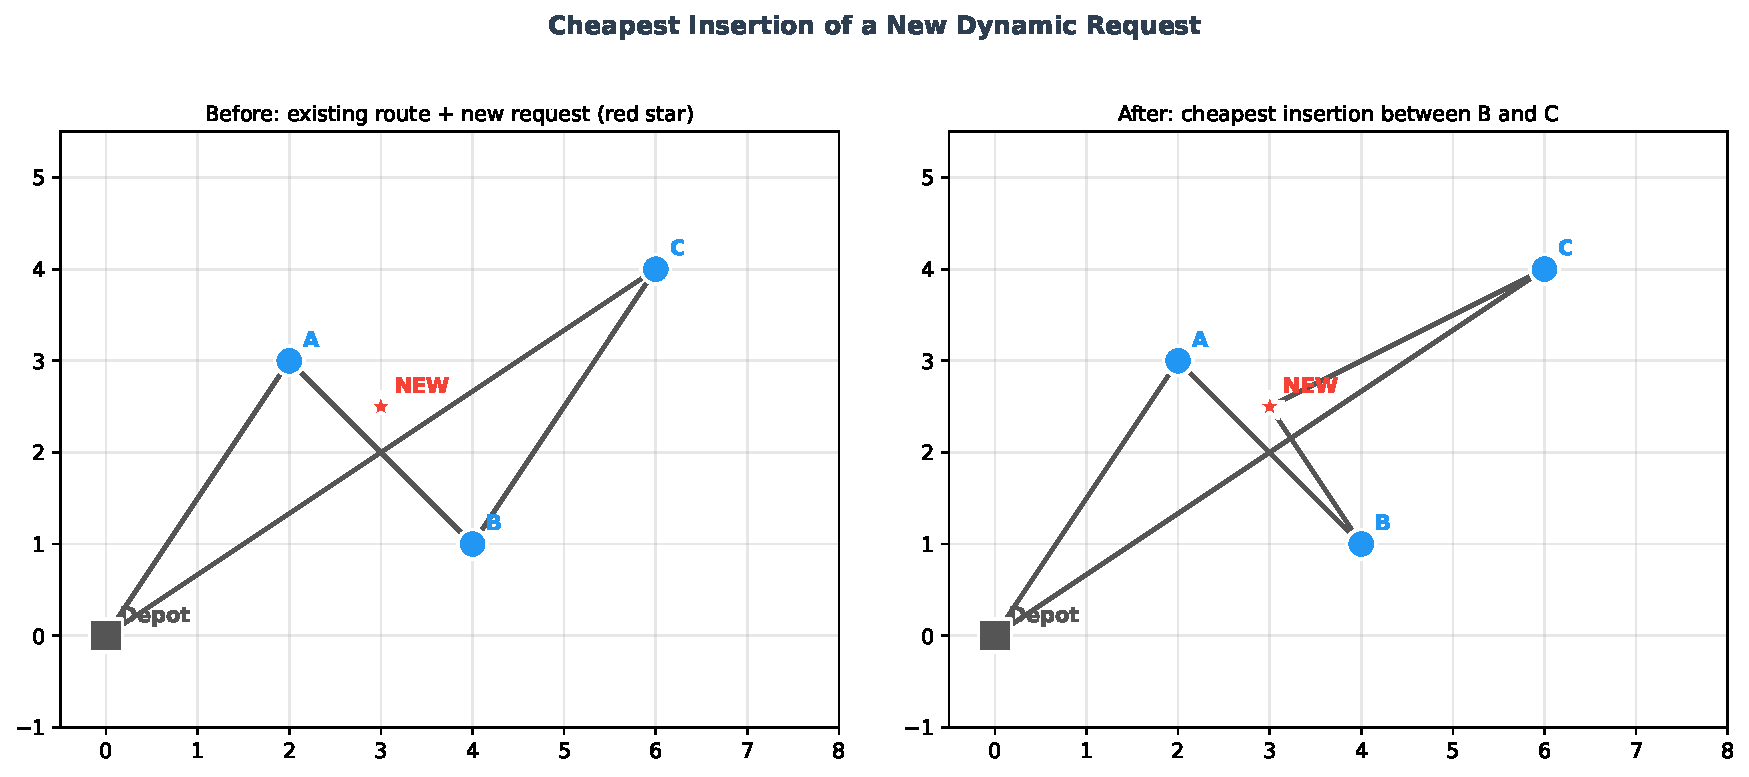
\includegraphics[width=0.88\textwidth]{ch11_insertion_heuristic.pdf}
    \caption{Cheapest insertion of a new dynamic request (red star) into an
             existing route.  The algorithm evaluates inserting the new customer
             between every consecutive pair of nodes and selects the insertion
             with minimum added distance.}
  \end{figure}

  \framebreak

  \begin{block}{Pseudocode: Cheapest Insertion for a Dynamic Request}
    \textbf{Input:} Current route plan $R = (r_1, r_2, \ldots, r_K)$ for $K$ vehicles;
    new request $c$ with location $p_c$, demand $q_c$, time window $[e_c, l_c]$.\\
    \textbf{Output:} Updated route plan with $c$ inserted.

    \medskip
    \begin{enumerate}
      \item Set $\Delta^* \leftarrow +\infty$; best vehicle $k^* \leftarrow \text{none}$;
            best position $\text{pos}^* \leftarrow \text{none}$.
      \item \textbf{For each} vehicle $k \in \{1, \ldots, K\}$:
        \begin{enumerate}
          \item Check remaining capacity: if $Q_k^{\mathrm{rem}} < q_c$, skip this vehicle.
          \item \textbf{For each} consecutive pair $(i, j)$ in route $r_k$:
            \begin{enumerate}
              \item Compute $\Delta = d(i, c) + d(c, j) - d(i, j)$.
              \item Check time-window feasibility of inserting $c$ between $i$ and $j$.
              \item If feasible and $\Delta < \Delta^*$: set $\Delta^* \leftarrow \Delta$,
                    $k^* \leftarrow k$, $\text{pos}^* \leftarrow (i, j)$.
            \end{enumerate}
        \end{enumerate}
      \item If $\Delta^* < +\infty$: insert $c$ between $i$ and $j$ in route $r_{k^*}$.
      \item Else: $c$ cannot be served (reject or add emergency vehicle).
    \end{enumerate}
  \end{block}

  \begin{alertblock}{Key insight}
    The time complexity of cheapest insertion is $O(K \cdot n)$ where $n$ is
    the total number of stops across all routes.  For typical fleet sizes this
    is fast enough to run in real time.
  \end{alertblock}

\end{frame}

% ────────────────────────────────────────────────────────────
\begin{frame}[allowframebreaks]{Periodic Re-optimisation — Rolling Horizon}

  Instead of reacting to each individual request, a \textbf{rolling horizon}
  approach re-solves the complete routing problem at regular time intervals
  $\Delta t$.  At each planning epoch (that is, each interval boundary), the
  dispatcher collects all requests that have arrived since the last
  re-optimisation and solves a new VRP that integrates both old (not-yet-served)
  and new customers.

  \begin{figure}
    \centering
    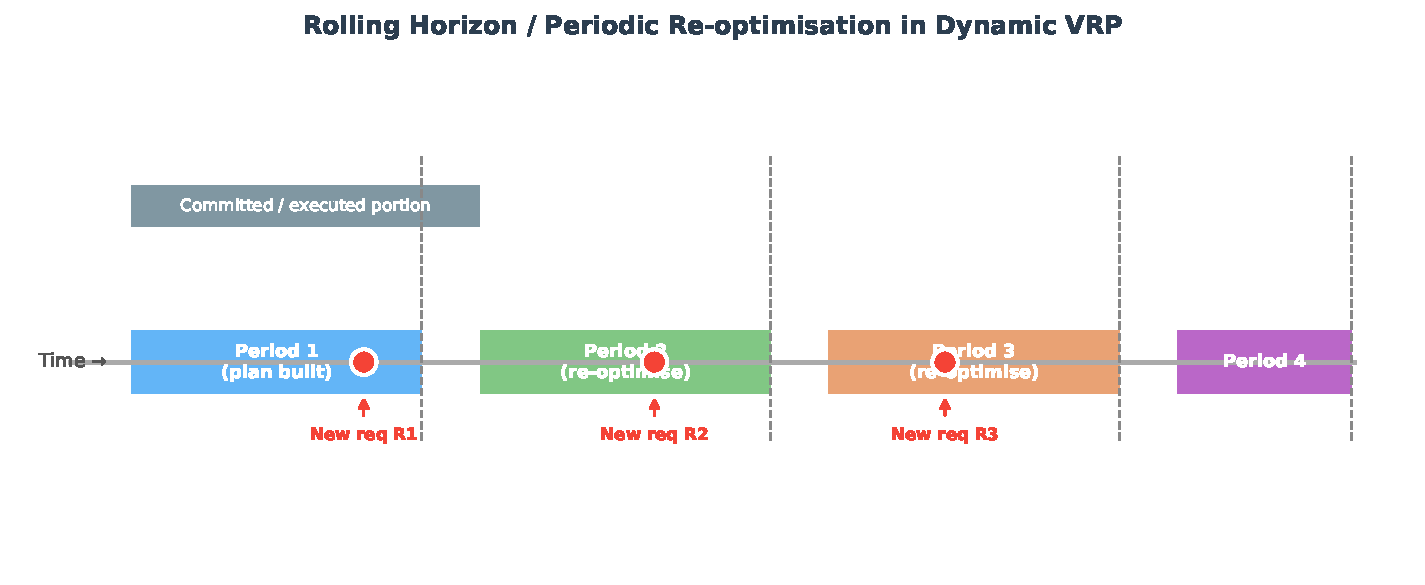
\includegraphics[width=0.88\textwidth]{ch11_rolling_horizon.pdf}
    \caption{Rolling horizon re-optimisation.  The grey bar shows the portion of
             the route that has already been committed (vehicles are already
             en route to those customers).  At each period boundary, new
             requests (red dots) are incorporated and the remaining plan is
             re-optimised.}
  \end{figure}

  \framebreak

  \begin{block}{Rolling Horizon — Algorithm}
    \textbf{Input:} Set of a priori requests $C^0$; re-planning interval $\Delta t$.\\
    \textbf{Output:} Sequence of route plans $P^0, P^1, P^2, \ldots$

    \medskip
    \begin{enumerate}
      \item At $t = 0$: compute initial plan $P^0$ using all $C^0$ requests.
            Dispatch vehicles according to $P^0$.
      \item \textbf{Repeat} at each epoch $t = \Delta t, 2\Delta t, 3\Delta t, \ldots$:
        \begin{enumerate}
          \item Collect all new requests $C^{\mathrm{new}}$ that arrived in
                the interval $(t - \Delta t, t]$.
          \item Freeze all vehicle actions that have already been committed
                (stops already begun or past their re-routing deadline).
          \item Re-solve the VRP on the remaining (uncommitted) customer set
                plus $C^{\mathrm{new}}$, using current vehicle positions as
                new depots.
          \item Update the active plan; continue vehicle dispatch.
        \end{enumerate}
    \end{enumerate}
  \end{block}

  \begin{alertblock}{Trade-off: $\Delta t$ choice}
    A small $\Delta t$ (frequent re-planning) adapts quickly to new requests
    but uses more computational resources and may disrupt vehicle plans
    frequently.  A large $\Delta t$ is computationally cheap but may serve
    requests late or produce routes that are difficult to improve once many
    requests have accumulated.  In practice, $\Delta t$ between 5 and 30
    minutes is common for courier applications.
  \end{alertblock}

\end{frame}

% ────────────────────────────────────────────────────────────
\begin{frame}[allowframebreaks]{Anticipatory Methods — Looking Ahead}

  Anticipatory algorithms go beyond reacting to what is currently known.
  They use \emph{probabilistic models} of future request arrivals to make
  better routing decisions today.  The underlying logic is: ``if I know
  that customers tend to appear in the eastern part of the city during the
  afternoon, I should position an idle vehicle there, even if no specific
  request has yet arrived.''

  \begin{figure}
    \centering
    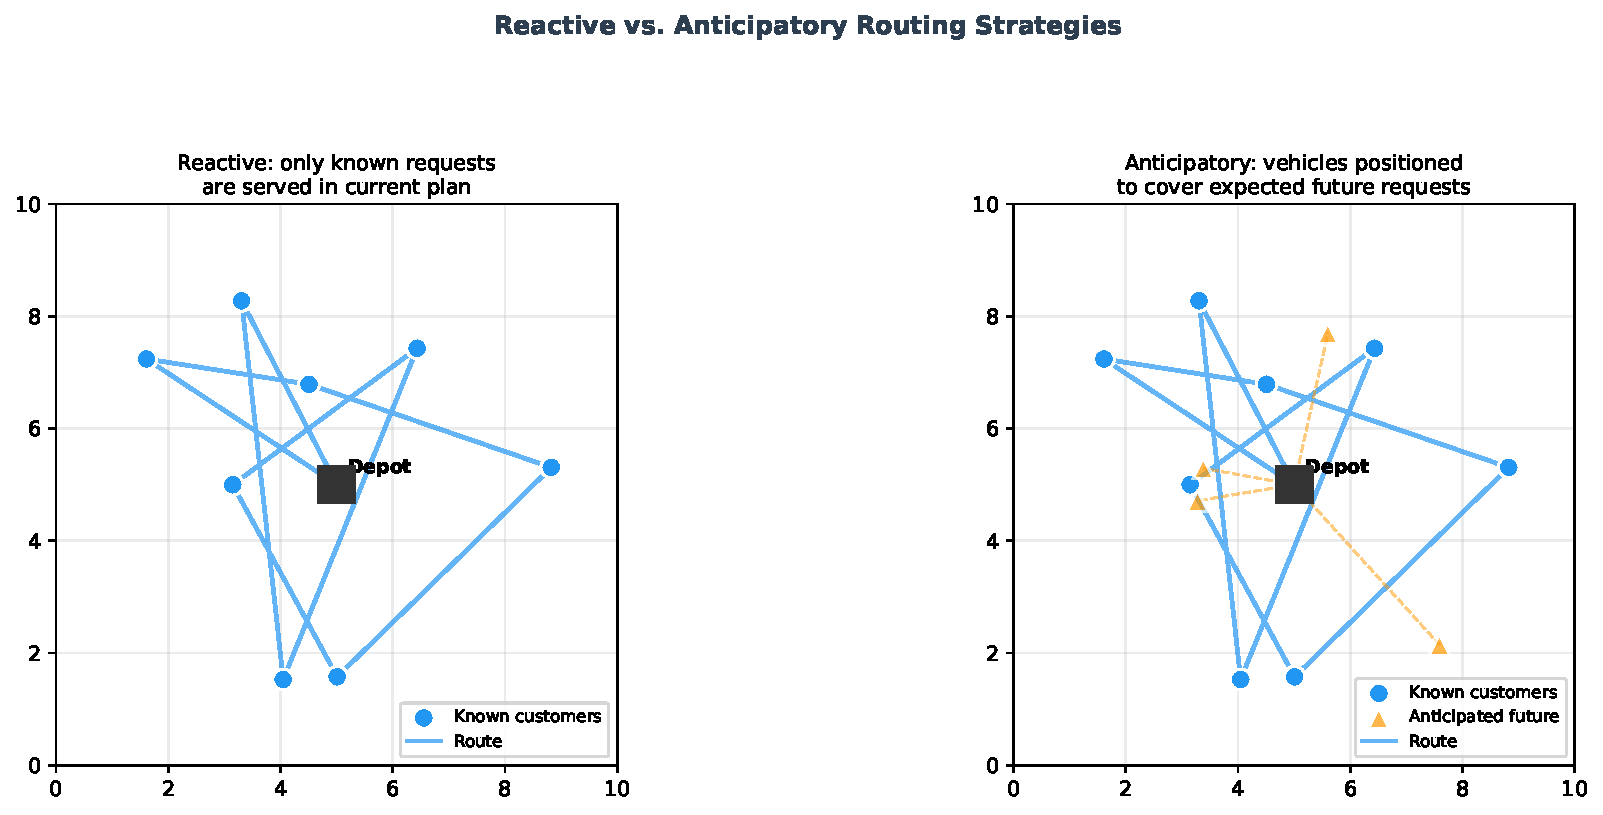
\includegraphics[width=0.88\textwidth]{ch11_reactive_vs_anticipatory.pdf}
    \caption{Reactive routing (left) only plans for currently known customers.
             Anticipatory routing (right) also considers likely future request
             locations (orange triangles) and positions vehicles accordingly,
             reducing total travel distance when those requests materialise.}
  \end{figure}

  \framebreak

  \begin{block}{Key idea — Anticipatory routing}
    Anticipatory routing algorithms maintain a probabilistic model of future
    request arrivals.  This model is typically a spatial--temporal distribution
    $\lambda(x, y, t)$ (lambda, read ``lambda'') giving the probability density
    of a new request arriving at location $(x, y)$ at time $t$.
    The algorithm then optimises not just over confirmed requests, but over
    the \emph{expected future cost}, which accounts for both current requests
    and the likely cost of serving future requests.
  \end{block}

  \begin{block}{Expected Future Cost}
    Let $\mathbb{E}[C_{\mathrm{future}}(\pi, t)]$ denote the expected cost of
    serving all future requests given that the current routing plan is $\pi$
    (pi, the Greek letter for the ratio of a circle's circumference to its
    diameter, here used as a general symbol for a plan) and the current time
    is $t$.  An anticipatory algorithm selects the plan $\pi^*$ that minimises:
    \[
      \pi^* = \arg\min_{\pi} \left[C_{\mathrm{current}}(\pi) +
              \gamma \cdot \mathbb{E}[C_{\mathrm{future}}(\pi, t)]\right]
    \]
    where $C_{\mathrm{current}}(\pi)$ is the cost of serving currently known
    requests under plan $\pi$, and $\gamma$ (gamma, a Greek letter used here
    as a weighting factor) controls the relative importance of future costs
    versus current costs.
  \end{block}

  \begin{block}{Notation}
    $\pi$ = current route plan (a complete assignment of customers to vehicles
    with a specified visit sequence); $C_{\mathrm{current}}(\pi)$ = total
    distance driven to serve all currently known customers under plan $\pi$;
    $\mathbb{E}[\cdot]$ = mathematical expectation (average over all possible
    future scenarios); $\gamma$ = weight on future costs, typically chosen by
    cross-validation on historical data.
  \end{block}

\end{frame}

% ────────────────────────────────────────────────────────────
\begin{frame}[allowframebreaks]{Routing Policies — No Wait, Wait, and Optimal}

  A crucial decision in dynamic routing is what to do with a vehicle that has
  just finished serving its currently assigned customers and is waiting for
  new requests.  Three broad policies are used:

  \begin{block}{No-Wait Policy}
    The vehicle immediately returns to the depot and waits there for the next
    dispatch instruction.  This policy is simple and ensures capacity is always
    available, but it wastes travel time if new requests arrive in areas far
    from the depot.
  \end{block}

  \begin{block}{Wait-at-Last-Customer Policy}
    The vehicle remains at the location of its last customer until a new
    request arrives or until it is recalled.  This avoids the return-trip
    cost but positions the vehicle at a location that may not be well-suited
    for future requests.
  \end{block}

  \begin{block}{Optimal Waiting (Anticipatory Policy)}
    The vehicle moves to a \emph{waiting position} that minimises the expected
    cost of serving future requests.  The waiting position is computed by
    solving a sub-problem: ``given the probability distribution of future
    requests, which location minimises expected additional travel?''
    Commonly, the optimal waiting position is the centroid (weighted average
    location) of the area where future requests are most likely to occur.
  \end{block}

  \framebreak

  \begin{figure}
    \centering
    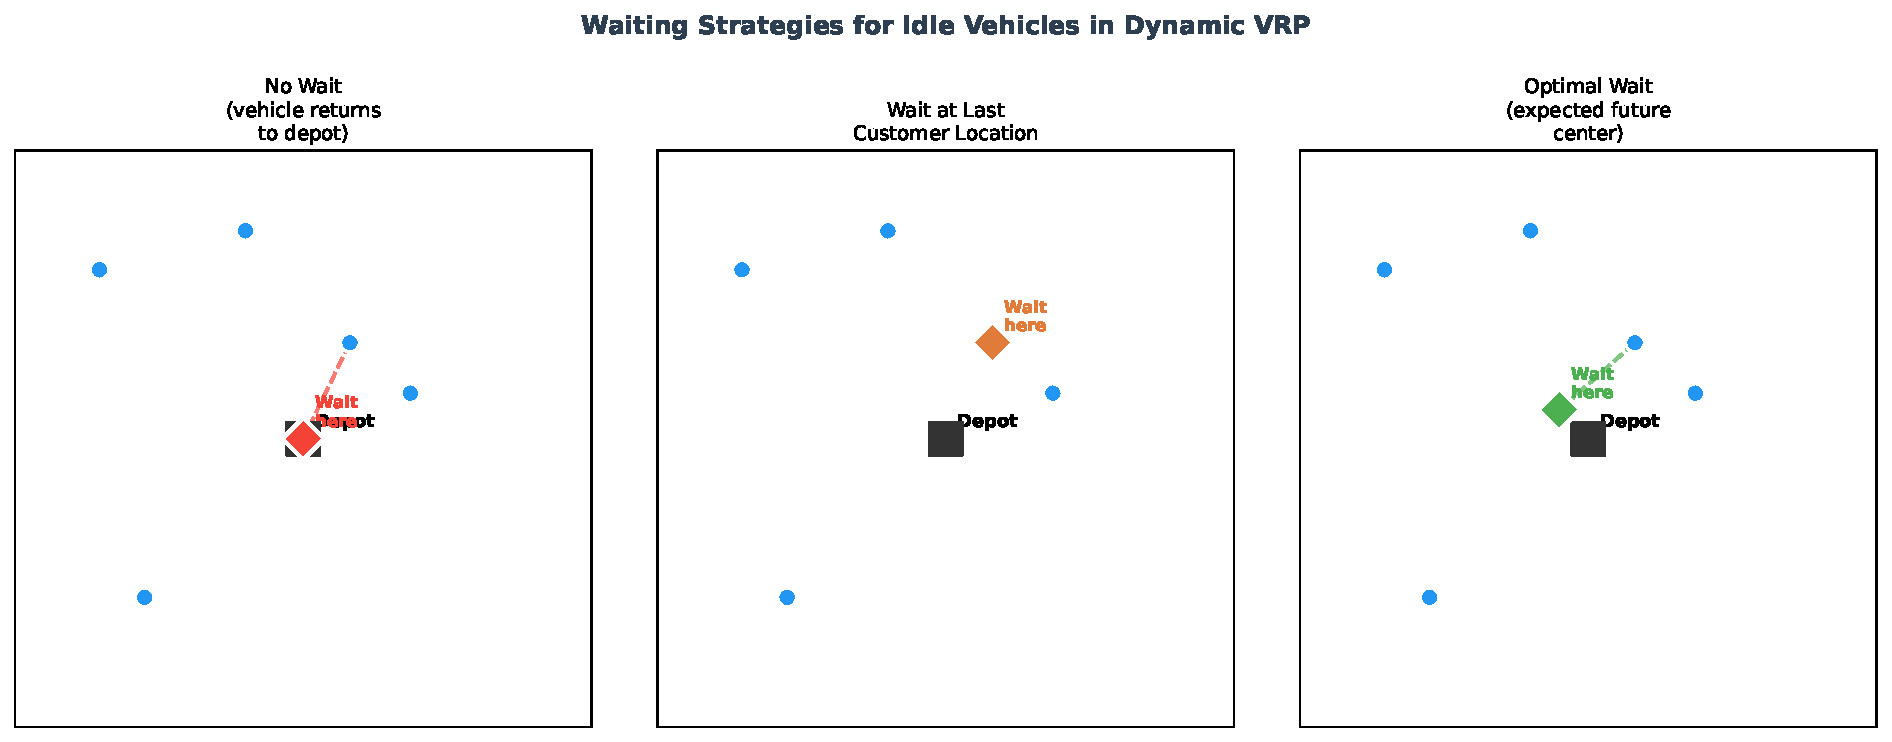
\includegraphics[width=0.88\textwidth]{ch11_waiting_strategies.pdf}
    \caption{Three waiting strategies for an idle vehicle (diamond marker).
             No-Wait (left): vehicle returns to depot.  Wait-at-Last (centre):
             vehicle stays at the final served location.  Optimal-Wait (right):
             vehicle moves to a position that minimises expected travel to
             future requests.}
  \end{figure}

  \framebreak

  Secomandi~(2000) showed that the simple no-wait policy is often surprisingly
  competitive, especially when the depot is centrally located.  However, for
  problems with clustered future request distributions, the optimal waiting
  position can substantially outperform both the no-wait and wait-at-last
  policies.

  \begin{alertblock}{Key insight}
    The benefit of an intelligent waiting policy is largest when (i) travel
    times are high relative to service times, (ii) future requests cluster
    spatially away from the depot, and (iii) the algorithm has accurate
    information about where future requests are likely to appear.
    If the spatial distribution of requests is unknown or uniform, the
    no-wait policy performs as well as more sophisticated alternatives.
  \end{alertblock}

\end{frame}

% ────────────────────────────────────────────────────────────
\begin{frame}[allowframebreaks]{Sampling-Based Anticipatory Algorithms}

  One of the most effective classes of anticipatory algorithms uses
  \textbf{Monte Carlo sampling} to generate multiple scenarios of future
  request arrivals and averages the optimisation results across those scenarios.
  This approach was pioneered by Bent and Van Hentenryck~(2004) for the
  dynamic VRPTW.

  \begin{block}{Core idea — Multiple Scenario Optimisation (MSO)}
    At each decision point (that is, whenever a new request arrives or a
    vehicle becomes idle), the algorithm:
    \begin{enumerate}
      \item Generates $S$ sample scenarios of future requests, drawn from
            a probabilistic model of arrivals.
      \item For each scenario $s \in \{1, \ldots, S\}$, solves the combined
            VRP on the union of known requests and the sampled future requests.
      \item Selects the \emph{immediate action} (which vehicle goes where next)
            that is best on average across all $S$ scenarios.
      \item Executes that immediate action; waits for the next event.
    \end{enumerate}
  \end{block}

  \begin{block}{Mathematical statement}
    Let $\omega_s$ (omega sub s) be scenario $s$ — a sampled set of future
    requests.  Let $f(\pi, \omega_s)$ be the cost of plan $\pi$ when future
    requests $\omega_s$ materialise.  The algorithm selects the plan:
    \[
      \pi^* = \arg\min_{\pi} \frac{1}{S} \sum_{s=1}^{S} f(\pi, \omega_s)
    \]
    where the sum $\sum_{s=1}^{S}$ runs over all $S$ sampled scenarios.
  \end{block}

  \begin{block}{Notation}
    $S$ = number of sample scenarios (typically 10 to 1000); $\omega_s$
    (omega sub s) = one sampled realisation of future requests;
    $f(\pi, \omega_s)$ = objective value of plan $\pi$ if scenario $\omega_s$
    occurs; the fraction $1/S$ averages over all scenarios.
  \end{block}

  \begin{alertblock}{Why this works}
    By averaging over many scenarios, the algorithm identifies actions that
    are \emph{robustly good} — they work well under a wide range of possible
    futures, not just under the current best guess.  This hedging behaviour
    is what distinguishes anticipatory methods from purely reactive ones.
  \end{alertblock}

  \framebreak

  \begin{figure}
    \centering
    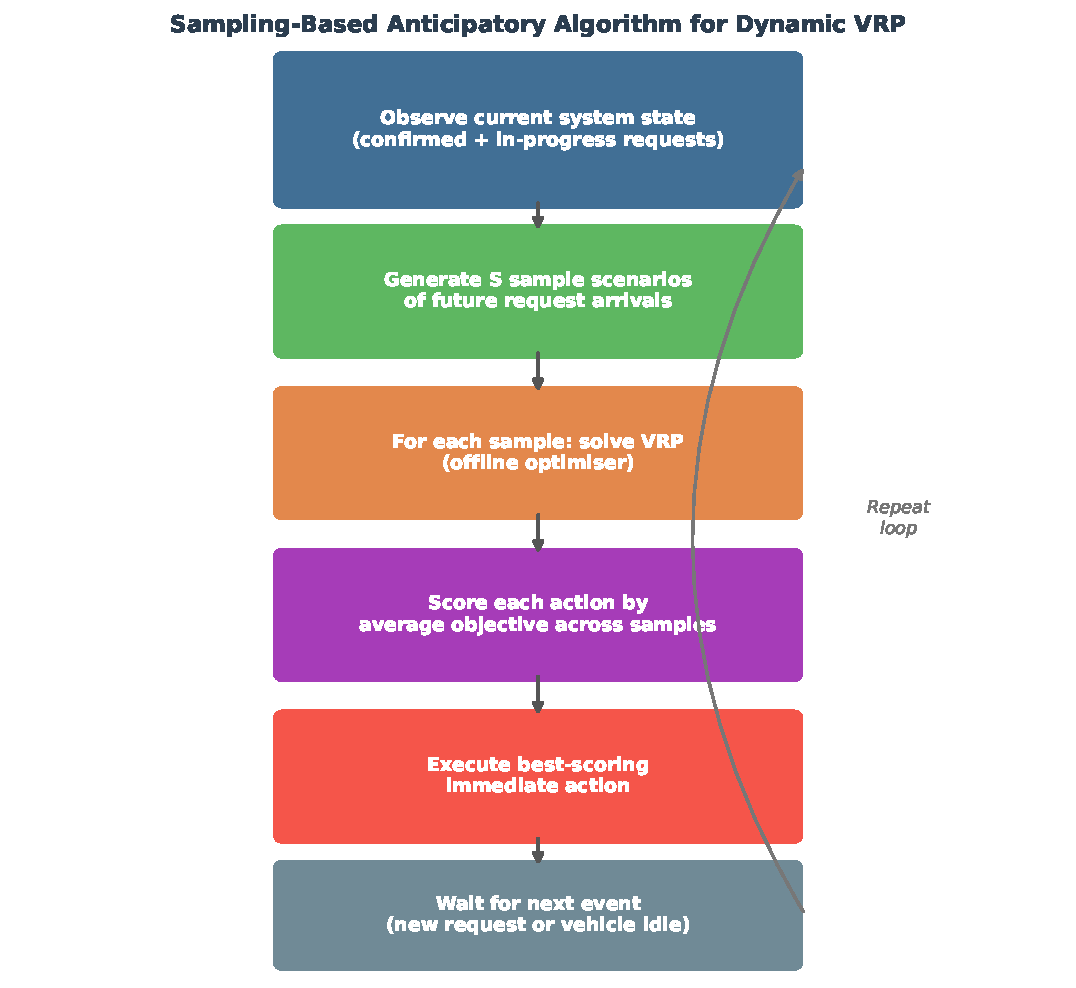
\includegraphics[width=0.75\textwidth]{ch11_sampling_algorithm.pdf}
    \caption{Flowchart of the sampling-based anticipatory algorithm.
             The outer loop repeats whenever the system state changes
             (new request or vehicle event).  Each iteration samples
             future scenarios, solves a VRP for each, and executes only
             the best immediate action.}
  \end{figure}

  \framebreak

  \begin{block}{Survey of sampling approaches from the literature}
    \begin{tabular}{p{3.5cm}p{5.5cm}p{4.5cm}}
      \toprule
      Reference & Problem & Key contribution\\
      \midrule
      Bent \& Van Hentenryck (2004) & Dynamic VRPTW & MSO with multiple plan approach; showed sampling outperforms re-insertion\\
      Flatberg et al.\ (2005) & Dynamic VRP & Combined local search with scenario sampling\\
      Hvattum et al.\ (2006) & Dynamic VRPTW & Branch \& bound within each scenario\\
      Goodson et al.\ (2012) & Dynamic VRPTW & Rollout policy with value functions\\
      \bottomrule
    \end{tabular}
  \end{block}

  The work of Bent and Van Hentenryck is particularly notable.  Their
  \textbf{Multiple Plan (MP)} approach maintains a \emph{pool} of plans
  simultaneously rather than committing to a single plan.  At each event,
  plans in the pool that are infeasible or that do not serve a newly arrived
  customer are discarded; the surviving plans are re-optimised.  The vehicle
  executes the action that is common to the greatest number of surviving plans.
  This consensus-based approach naturally hedges against uncertainty without
  explicitly sampling from a probability model.

\end{frame}

% ────────────────────────────────────────────────────────────
\begin{frame}[allowframebreaks]{Metaheuristics for Dynamic VRP}

  Several metaheuristic algorithms originally developed for static VRP have
  been adapted to the dynamic setting.  The adaptations typically involve
  running the metaheuristic in a time-limited fashion between events, and
  using warm-starts (initialising from the previous solution) to exploit
  the fact that plans change incrementally rather than completely.

  \begin{block}{Tabu Search for Dynamic VRP}
    Tabu search maintains a \emph{tabu list} of recently visited solutions and
    forbids the search from returning to them.  In a dynamic setting, tabu
    search is run continuously in a background thread.  Whenever a new request
    arrives, it is added to the current best solution using cheapest insertion,
    and the tabu search then improves from that starting point.

    The analogy: tabu search is like a hiker exploring a hilly landscape,
    deliberately avoiding recently visited locations (tabu list) to escape
    local optima and explore new terrain.  In the dynamic setting, the
    landscape changes as new requests arrive, so the hiker must constantly
    adapt to new terrain whilst also trying to reach a better peak.
  \end{block}

  \begin{block}{Evolutionary Algorithms for Dynamic VRP}
    Genetic algorithms (GA) maintain a \textbf{population} of candidate solutions.
    In the dynamic VRP context, an evolutionary algorithm:
    \begin{enumerate}
      \item Maintains a population of feasible route plans.
      \item When a new request arrives, updates all population members by
            inserting the new customer at its cheapest position in each plan.
      \item Applies crossover and mutation operators to generate new candidate
            plans.
      \item Selects the best individuals for the next generation.
    \end{enumerate}
    Because a diverse population is maintained, the algorithm naturally hedges
    against uncertainty: some plans may serve the new request cheaply, others
    position vehicles well for future requests.
  \end{block}

  \framebreak

  Kilby, Prosser, and Shaw~(1998) proposed a dynamic programming approach
  for the dynamic VRPTW.  The state in their DP consists of the current
  vehicle positions and the set of pending requests.  Transitions correspond
  to vehicle dispatching decisions.  While the full DP is intractable for
  large instances, approximations and decompositions make it practical.

  \begin{block}{Dynamic Programming for Dynamic VRP — Bellman Equation}
    Let $V(s, t)$ denote the minimum expected total travel cost starting from
    state $s$ at time $t$, where $s$ encodes the positions of all vehicles and
    the set of unserved customers.  The Bellman equation is:
    \[
      V(s, t) = \min_{a \in A(s)} \left[ c(s, a) + \mathbb{E}[V(s', t')] \right]
    \]
    where $A(s)$ (A of s) is the set of feasible actions from state $s$,
    $a$ is one such action (a dispatch decision), $c(s, a)$ is the immediate
    cost of action $a$, and $s'$ is the next state reached after action $a$
    and any new arrivals during the transition.
  \end{block}

  \begin{block}{Notation}
    $V(s, t)$ = value function (minimum expected future cost from state $s$
    at time $t$); $A(s)$ = feasible action set; $c(s, a)$ = immediate travel
    cost of action $a$ in state $s$; $\mathbb{E}[V(s', t')]$ = expected
    future value after transitioning to state $s'$.
  \end{block}

  \begin{alertblock}{How to read the Bellman equation}
    The equation says: ``the best policy from state $s$ is to choose action
    $a$ that minimises the sum of (i) what you pay right now and (ii) the
    expected best cost from the next state onward.''  This recursive structure
    means that knowing $V$ at the next step is sufficient to make a greedy
    optimal decision at the current step — this is the \emph{principle of
    optimality}.
  \end{alertblock}

\end{frame}

% ────────────────────────────────────────────────────────────
\begin{frame}[fragile]{Python — Cheapest Insertion for Dynamic Request}

The following Python function implements the cheapest-insertion rule for
adding a new dynamic customer into an existing set of routes.  The function
checks capacity and time-window feasibility at each candidate insertion
position and returns the best (minimum extra cost) insertion.

\begin{lstlisting}
import math
from typing import List, Tuple, Optional

def distance(p1: Tuple[float, float], p2: Tuple[float, float]) -> float:
    """Euclidean distance between two (x, y) coordinate pairs."""
    return math.hypot(p1[0] - p2[0], p1[1] - p2[1])

def cheapest_insertion(
    routes: List[List[dict]],     # each route is a list of customer dicts
    new_customer: dict,           # {'id', 'x', 'y', 'demand', 'tw_open', 'tw_close'}
    vehicle_capacities: List[float],
    vehicle_loads: List[float],
) -> Optional[Tuple[int, int]]:
    """
    Find the cheapest feasible insertion of new_customer into routes.

    Returns (route_index, insert_after_index) or None if infeasible.
    insert_after_index = i means insert new_customer after position i
    in routes[route_index].
    """
    best_delta = float('inf')
    best_route, best_pos = None, None

    nc = new_customer
    nc_loc = (nc['x'], nc['y'])

    for k, route in enumerate(routes):
        # Check vehicle capacity
        remaining_cap = vehicle_capacities[k] - vehicle_loads[k]
        if remaining_cap < nc['demand']:
            continue   # cannot serve: insufficient capacity

        # Try inserting after each position in the route
        # route[0] = depot, route[-1] = return to depot
        for i in range(len(route) - 1):
            prev_node = route[i]
            next_node = route[i + 1]

            prev_loc = (prev_node['x'], prev_node['y'])
            next_loc = (next_node['x'], next_node['y'])

            # Extra distance cost of insertion
            delta = (distance(prev_loc, nc_loc)
                   + distance(nc_loc, next_loc)
                   - distance(prev_loc, next_loc))

            # Simplified time-window check
            # (arrival at new_customer must be within its time window)
            arr_nc = prev_node.get('departure', 0) + distance(prev_loc, nc_loc)
            if arr_nc > nc['tw_close']:
                continue   # violates time window

            if delta < best_delta:
                best_delta = delta
                best_route = k
                best_pos   = i

    if best_route is not None:
        return (best_route, best_pos)
    return None  # no feasible insertion found


# ── Example usage ──────────────────────────────────────────
depot = {'id': 0, 'x': 0.0, 'y': 0.0, 'demand': 0,
         'tw_open': 0, 'tw_close': 1440, 'departure': 0}

route1 = [
    depot,
    {'id': 1, 'x': 2.0, 'y': 3.0, 'demand': 5, 'tw_open':  60,
     'tw_close': 120, 'departure': 80},
    {'id': 2, 'x': 4.0, 'y': 1.0, 'demand': 3, 'tw_open':  90,
     'tw_close': 200, 'departure': 150},
    depot,
]
new_req = {'id': 99, 'x': 3.0, 'y': 2.5, 'demand': 2,
           'tw_open': 70, 'tw_close': 180}

result = cheapest_insertion(
    routes=[route1], new_customer=new_req,
    vehicle_capacities=[20.0], vehicle_loads=[8.0])
print("Best insertion:", result)
# Output: Best insertion: (0, 1)  -> insert after index 1 (after customer 1)
\end{lstlisting}

\end{frame}

% ────────────────────────────────────────────────────────────
\begin{frame}[allowframebreaks]{Analytical Studies — Dynamic VRP Literature Survey}

  Table~11.3 in the textbook (reproduced and summarised below) provides an
  overview of the major algorithmic approaches for dynamic VRP with requests,
  drawn from the published literature.  The table distinguishes approaches by
  the type of dynamic VRP addressed and the algorithmic family used.

  \begin{block}{Summary of key approaches for dynamic requests}
    \begin{tabular}{p{3.8cm}p{4.0cm}p{5.5cm}}
      \toprule
      Reference & Problem type & Algorithm\\
      \midrule
      Gendreau et al.\ (1999) & Dynamic VRPTW & Tabu search with double re-insertion\\
      Liao et al.\ (1992) & Dynamic PDP & Insertion with dispatch rules\\
      Taillard et al.\ (1996) & Dynamic VRP & Tabu search, adaptive memory\\
      Gendreau \& Potvin (1998) & Dynamic VRPTW & Branch \& bound with re-optimisation\\
      Bent \& Van Hentenryck (2004) & Dynamic VRPTW & Multiple plans, Monte Carlo\\
      Hvattum et al.\ (2006) & Dynamic VRPTW & Branch \& bound per scenario\\
      Wen et al.\ (2010) & Dynamic VRPTW & Adaptive large neighbourhood search\\
      Goodson et al.\ (2012) & Dynamic VRPTW & Rollout, DP approximation\\
      \bottomrule
    \end{tabular}
  \end{block}

  \framebreak

  The work of Gendreau, Guertin, Potvin, and Seguin~(1999) is a landmark in
  dynamic VRP research.  They proposed a \textbf{tabu search} algorithm
  specifically designed for dynamic VRPTW, running continuously in real time.
  Their double re-insertion move simultaneously relocates two customers,
  which is more powerful than single-customer re-insertions but still fast
  enough for online use.

  Taillard et al.~(1996) introduced the concept of \textbf{adaptive memory}
  programming, where high-quality partial routes found in previous planning
  cycles are stored and reused in future optimisations.  This is particularly
  effective in rolling horizon settings where routes change only incrementally
  between epochs.

  Wen et al.~(2010) proposed an \textbf{adaptive large neighbourhood search}
  (ALNS) for dynamic VRPTW.  ALNS combines multiple \emph{destroy operators}
  (which remove a subset of customers from routes) with \emph{repair operators}
  (which reinsert those customers).  The algorithm adaptively selects which
  operators to use based on their historical performance, making it
  self-tuning over the course of a single run.

\end{frame}

% ============================================================
\section{Dynamic and Time-Dependent Travel Times}
% ============================================================

\begin{frame}[allowframebreaks]{Dynamic Travel Times — Congestion and Variability}

  In real-world transportation networks, travel times are not constant.
  They depend on the \textbf{time of day} (due to rush-hour congestion),
  on \textbf{day-of-week effects}, on \textbf{weather}, and on
  \textbf{incidents} such as accidents or road closures.  Algorithms that
  ignore this variability and use fixed travel times may produce routes that
  violate time windows in practice or that are significantly sub-optimal.

  \begin{block}{Time-Dependent Travel Time Model}
    Let $t_{ij}(\tau)$ (t sub ij of tau, where $\tau$ (tau) is the departure
    time) be the travel time from node $i$ to node $j$ when departure occurs
    at time $\tau$.  In the simplest model, travel times are piecewise-linear
    functions of departure time:
    \[
      t_{ij}(\tau) = \frac{d_{ij}}{v_{ij}(\tau)}
    \]
    where $d_{ij}$ is the fixed distance from $i$ to $j$ and $v_{ij}(\tau)$
    (v sub ij of tau) is the average speed on that arc at departure time $\tau$.
  \end{block}

  \begin{block}{Notation}
    $t_{ij}(\tau)$ = travel time from $i$ to $j$ when leaving $i$ at time $\tau$;
    $d_{ij}$ = fixed geographic distance (km); $v_{ij}(\tau)$ = speed (km/h) on
    arc $(i,j)$ at departure time $\tau$; $\tau$ (tau, Greek letter) = clock
    time of departure.
  \end{block}

  \begin{alertblock}{How to read this formula}
    Think of $t_{ij}(\tau)$ as a travel-time function rather than a single
    number.  If you leave node $i$ at 8~am when rush hour is in full swing,
    $v_{ij}(8\text{h})$ is low (say, 20~km/h in heavy traffic), so the
    travel time is high.  If you leave at 11~am, $v_{ij}(11\text{h})$ might
    be 60~km/h, giving one-third the travel time.
    Routing algorithms that account for this dependency can save substantial
    time by scheduling stops in a sequence that avoids peak congestion.
  \end{alertblock}

  \framebreak

  \begin{figure}
    \centering
    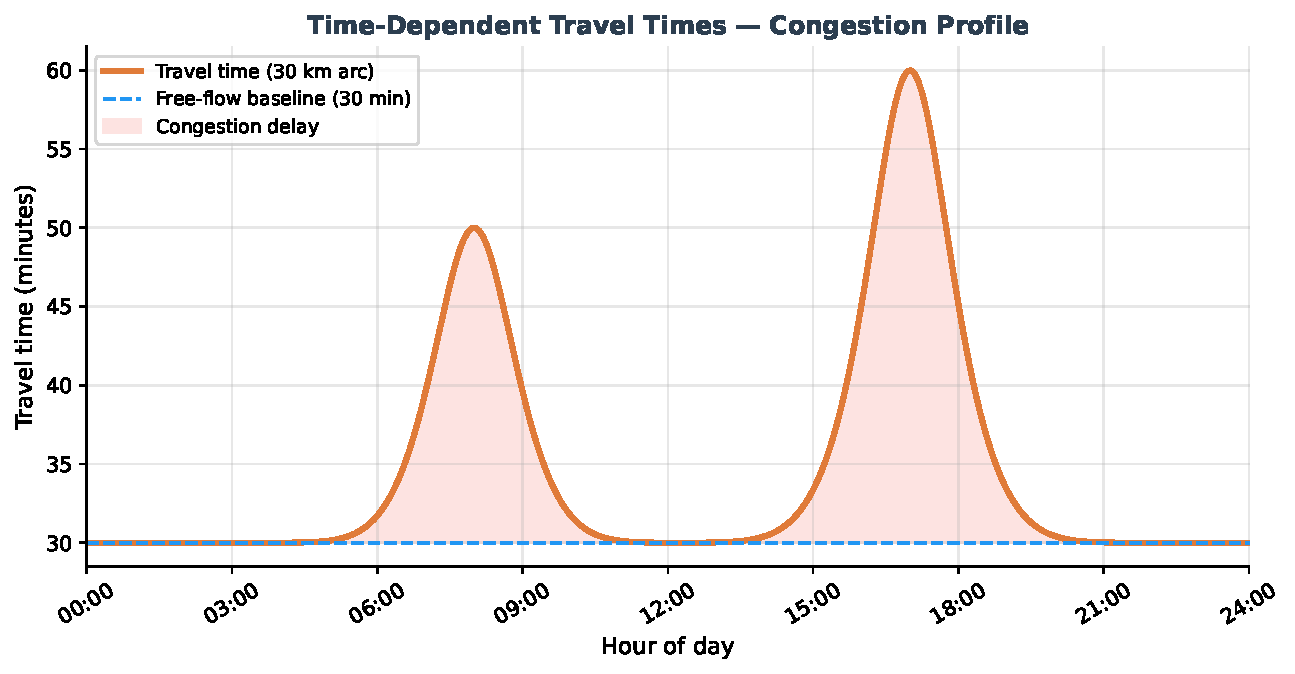
\includegraphics[width=0.88\textwidth]{ch11_time_dependent_travel.pdf}
    \caption{Illustration of time-dependent travel times for a fixed 30~km arc.
             Morning and evening rush hours create two congestion peaks, raising
             the travel time from 30~minutes (free-flow baseline, blue dashed)
             to nearly 50~minutes.  The red shaded area shows the additional
             delay due to congestion.}
  \end{figure}

  \framebreak

  \begin{block}{FIFO Property (First In, First Out)}
    A time-dependent travel time function satisfies the \textbf{FIFO property}
    if leaving later never allows you to arrive earlier:
    \[
      \tau_1 < \tau_2 \implies \tau_1 + t_{ij}(\tau_1) \leq \tau_2 + t_{ij}(\tau_2)
    \]
    In words: if vehicle A departs before vehicle B on the same arc, then
    vehicle A arrives no later than vehicle B.  The FIFO property ensures
    that shortest-path algorithms like Dijkstra's algorithm generalise
    correctly to time-dependent networks.
  \end{block}

  \begin{alertblock}{Why FIFO matters}
    Most standard shortest-path algorithms assume that waiting is always
    free (you can always wait and then travel).  If the FIFO property holds,
    then a vehicle that departs earlier always arrives no later, which means
    there is never any benefit to deliberately delaying departure.  Without
    the FIFO property, route planning becomes significantly more complex
    because optimal solutions might involve deliberate waiting at intermediate
    nodes.
  \end{alertblock}

  \framebreak

  Several algorithmic approaches for the time-dependent VRP (TDVRP) have been
  proposed:

  \begin{block}{Algorithms for TDVRP}
    \begin{enumerate}
      \item \textbf{Adapted Clarke-Wright savings.}  The savings algorithm is
            modified so that the saving $s_{ij}$ for merging two routes at
            nodes $i$ and $j$ accounts for the time-dependent travel time
            at the estimated departure time.
      \item \textbf{Tabu search with time-dependent cost evaluation.}
            Standard VRP tabu search, but whenever a move is evaluated,
            the route is re-evaluated using $t_{ij}(\tau)$ for the actual
            departure time at each arc.
      \item \textbf{Evolutionary algorithms.}  Genetic algorithms with
            time-dependent cost functions embedded in the objective
            function evaluation.
    \end{enumerate}
  \end{block}

  Ichoua, Gendreau, and Potvin~(2003) provide a comprehensive study of
  time-dependent VRP.  They model speed as a step function of time
  (constant speed within each time interval) and show that incorporating
  time-dependency substantially reduces both total travel time and
  time-window violations compared with static routing.

  Maden, Eglese, and Black~(2010) validated time-dependent VRP approaches
  using real road network data from the UK, demonstrating practical savings
  of 5--15\% in total travel time when congestion is explicitly modelled.

  Huang, Chen, and Chang~(2014) proposed a dynamic VRP with both time-dependent
  travel times and online requests, integrating a congestion model with
  a rolling-horizon re-optimisation framework.  Their computational results
  confirm that ignoring time dependency leads to systematic route infeasibility
  during peak hours.

\end{frame}

% ============================================================
\section{Dynamic Vehicle Availability}
% ============================================================

\begin{frame}[allowframebreaks]{Dynamic Vehicle Availability — Breakdowns and Windows}

  A further source of dynamism arises from the vehicles themselves rather
  than from customers or the road network.  In practice, a vehicle may:
  \begin{itemize}
    \item \textbf{Break down} mid-route, requiring emergency retrieval and
          redistribution of its remaining customers to other vehicles.
    \item \textbf{Become available late}, for example because it was used
          the previous evening and needs to return from a remote depot.
    \item \textbf{Have a restricted time window} during which it may operate,
          such as when a driver has contractual duty-time limits.
  \end{itemize}

  \begin{figure}
    \centering
    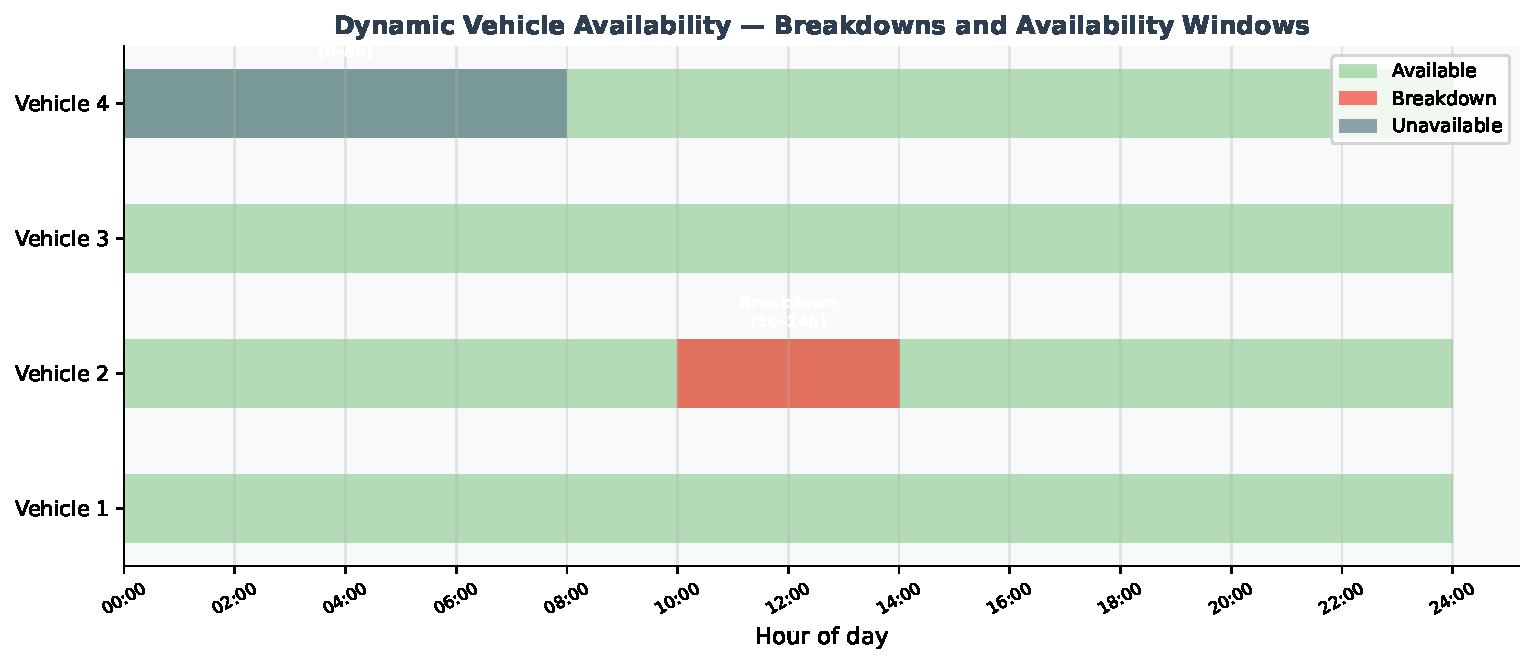
\includegraphics[width=0.86\textwidth]{ch11_vehicle_availability.pdf}
    \caption{Dynamic vehicle availability: Vehicle~2 suffers a breakdown
             from 10:00 to 14:00; Vehicle~4 is not available until 08:00.
             Algorithms must re-assign the affected customers to other
             vehicles in real time.}
  \end{figure}

  \framebreak

  \begin{block}{Problem Formulation — Vehicle Breakdown}
    When vehicle $k$ breaks down at time $t_b$ (t sub b) at location $\ell$
    (ell, representing a position), the remaining unserved customers $U_k$ in
    its route must be reassigned.  The sub-problem is:

    \medskip
    \textbf{Given:} Current positions of all vehicles $k' \neq k$;
    remaining loads and route plans of vehicles $k' \neq k$;
    the set of unserved customers $U_k$ from the broken-down vehicle.

    \medskip
    \textbf{Find:} An assignment of customers in $U_k$ to vehicles $k' \neq k$
    such that:
    \begin{itemize}
      \item Capacity constraints of all vehicles are maintained.
      \item Time-window constraints of all customers are maintained.
      \item The total additional distance driven is minimised.
    \end{itemize}

    This sub-problem is itself a VRP with fixed starting positions and is
    solved using the same heuristics as those for dynamic request insertion.
  \end{block}

  \framebreak

  Berbeglia, Cordeau, and Laporte~(2010) provide a comprehensive review of
  vehicle breakdown models in dynamic VRP.  They distinguish two sub-cases:

  \medskip
  \textbf{Soft breakdown:} The vehicle can continue operating, but at reduced
  capacity or speed.  The problem reduces to re-optimising routes with
  modified vehicle parameters.

  \medskip
  \textbf{Hard breakdown:} The vehicle is completely inoperable.  All remaining
  customers must be reassigned immediately.

  \begin{block}{Emergency vehicle dispatch as a special case}
    Emergency vehicle routing (ambulances, fire trucks) combines dynamic
    requests with dynamic vehicle availability.  Calls arrive randomly,
    must be served within tight time limits, and vehicles may be deployed
    (temporarily unavailable) for extended periods.  Liu, Madden, and
    Beibel~(2004) study this problem and show that preemptive redeployment
    strategies (repositioning free vehicles anticipatorily) can substantially
    reduce mean response times.
  \end{block}

  \begin{alertblock}{Key insight}
    The correct response to a vehicle breakdown in a dynamic VRP depends on
    how far from the depot the breakdown occurs and how many customers remain
    unserved.  If only one or two customers remain, it may be cheaper to send
    an entirely new vehicle.  If many customers remain and other vehicles are
    nearby, redistribution is preferred.  A fast feasibility check and a
    cheapest-insertion heuristic are typically sufficient for real-time response.
  \end{alertblock}

\end{frame}

% ────────────────────────────────────────────────────────────
\begin{frame}[allowframebreaks]{Vehicle Re-routing after Breakdown — Algorithm}

  \begin{block}{Re-routing Algorithm after Breakdown}
    \textbf{Input:} Broken-down vehicle $k$; remaining customer set $U_k$;
    current positions and plans of active vehicles $k' \in K \setminus \{k\}$.\\
    \textbf{Output:} Updated route plans for all active vehicles.

    \medskip
    \begin{enumerate}
      \item Sort customers in $U_k$ by urgency:
            those with tight time windows first.
      \item \textbf{For each} customer $c \in U_k$ in priority order:
        \begin{enumerate}
          \item Apply cheapest feasible insertion across all active vehicles.
          \item If insertion is feasible: add $c$ to that vehicle's plan.
          \item If no feasible insertion exists:
                \begin{itemize}
                  \item Attempt rerouting (remove a less-urgent customer
                        from another route to make room).
                  \item If still infeasible: flag $c$ as unserved and alert dispatcher.
                \end{itemize}
        \end{enumerate}
      \item Re-optimise each affected route using a local search (e.g., 2-opt)
            to recover any unnecessary detours introduced by insertions.
    \end{enumerate}
  \end{block}

  \begin{alertblock}{Practical note}
    Step~3 (local search improvement) is optional but important.  Simple
    cheapest insertion can produce routes with unnecessary ``zigzags'' because
    each insertion is made independently.  Running a quick 2-opt improvement
    pass after all insertions typically reduces total distance by 5--15\%.
  \end{alertblock}

\end{frame}

% ============================================================
\section{Performance Measurement and Evaluation}
% ============================================================

\begin{frame}[allowframebreaks]{Benchmarking Dynamic VRP Algorithms}

  Measuring the quality of a dynamic VRP algorithm is considerably more
  complex than measuring a static VRP algorithm.  In a static VRP, a single
  optimal solution (or a known lower bound) can serve as the benchmark.
  In a dynamic VRP, the set of customers is not known at the start of
  execution, making a direct comparison to an ``optimal'' solution difficult.

  \begin{block}{The Offline Optimal as a Benchmark}
    The most common benchmark for dynamic VRP algorithms is the
    \textbf{offline optimal}: the cost of the optimal solution to the
    \emph{static} VRP instance that includes \emph{all} customers —
    both a priori and dynamic — as if they had all been known in advance.

    \medskip
    Formally, let $Z^*_{\mathrm{offline}}$ be the optimal cost when all
    customer locations are known from the start.  Let $Z_{\mathrm{online}}(\mathcal{A})$
    be the cost achieved by online algorithm $\mathcal{A}$ that sees requests
    as they arrive.  The \textbf{online ratio} (or \emph{competitive ratio})
    of algorithm $\mathcal{A}$ is:
    \[
      \rho(\mathcal{A}) = \frac{Z_{\mathrm{online}}(\mathcal{A})}{Z^*_{\mathrm{offline}}}
    \]
  \end{block}

  \begin{block}{Notation}
    $Z^*_{\mathrm{offline}}$ = minimum cost achievable with perfect foresight;
    $Z_{\mathrm{online}}(\mathcal{A})$ = actual cost achieved by algorithm
    $\mathcal{A}$ under online conditions; $\rho(\mathcal{A})$ (rho, the Greek
    letter) = ratio of online to offline cost.  A value of $\rho = 1$ means the
    online algorithm performs as well as perfect-foresight planning (impossible
    in practice); a value of $\rho = 1.2$ means the online algorithm uses 20\%
    more distance than the theoretical offline optimum.
  \end{block}

  \begin{alertblock}{How to interpret $\rho$}
    The online ratio $\rho$ is always $\geq 1$ because the algorithm faces
    more uncertainty than the offline optimum.  Values of $\rho$ near 1 are
    desirable.  For highly dynamic problems (high dod), $\rho$ values of
    1.2--1.4 are typical even for the best known algorithms.
    For problems with low dod, good anticipatory algorithms can achieve
    $\rho$ very close to 1.
  \end{alertblock}

  \framebreak

  \begin{figure}
    \centering
    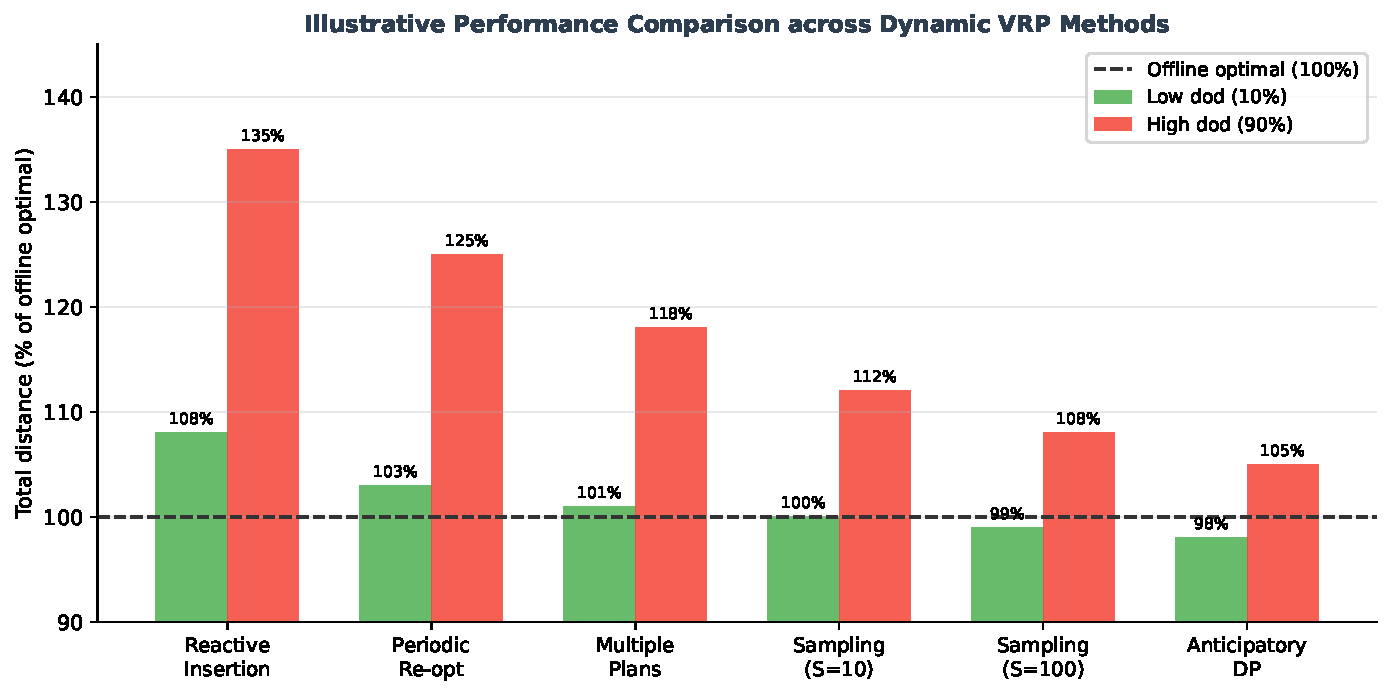
\includegraphics[width=0.88\textwidth]{ch11_benchmark_comparison.pdf}
    \caption{Illustrative performance comparison of dynamic VRP solution methods
             across two settings: low degree of dynamism (10\% dynamic requests,
             green bars) and high degree of dynamism (90\% dynamic requests,
             red bars).  All values are expressed as percentages of the offline
             optimal (100\%).  Sophisticated anticipatory methods offer larger
             advantages at low dod; at high dod the gap narrows.}
  \end{figure}

  \framebreak

  \begin{block}{Simulation-Based Evaluation}
    Because dynamic VRP performance depends on the realisation of random arrivals,
    a single-run comparison is unreliable.  Best practice is to evaluate
    algorithms over many \emph{randomly generated scenarios} using a consistent
    simulation framework.

    A simulation study typically proceeds as follows:
    \begin{enumerate}
      \item Fix a spatial distribution for customer locations (e.g., uniform
            on a $[0, 100]^2$ square, or clustered around $m$ centres).
      \item Fix an arrival-time distribution (e.g., Poisson with rate $\lambda$
            (lambda, read ``lambda'') requests per hour).
      \item Generate $N_{\mathrm{sim}}$ independent scenario realisations.
      \item For each realisation, run the dynamic VRP algorithm and record
            the cost $Z_{\mathrm{online}}^{(r)}$ for replicate $r$.
      \item Report the mean $\bar{Z} = \frac{1}{N_{\mathrm{sim}}} \sum_r Z_{\mathrm{online}}^{(r)}$
            and a 95\% confidence interval.
    \end{enumerate}
  \end{block}

  Larsen, Madsen, and Solomon~(2002, 2004) standardised the evaluation
  framework for dynamic VRPTW, proposing benchmark instance families based
  on Solomon's static VRPTW instances with additional dynamic components.
  These benchmarks have been widely adopted in subsequent research, making
  results comparable across different papers and research groups.

\end{frame}

% ────────────────────────────────────────────────────────────
\begin{frame}[allowframebreaks]{Tables from the Textbook — Algorithmic Overview}

  Tables~11.1 through~11.4 in the textbook systematically classify over
  60 papers on dynamic VRP.  The following summarises key dimensions of the
  classification:

  \begin{block}{Dimensions of the classification}
    \begin{tabular}{p{3.5cm}p{10cm}}
      \toprule
      Dimension & Values / categories\\
      \midrule
      Problem type & DVRP, D-VRPTW, D-DARP, D-PDP, emergency routing\\
      Objective     & Min distance, min vehicles, min rejections, min lateness\\
      dod range     & Low (${<}$30\%), medium (30--70\%), high (${>}$70\%)\\
      Algorithm     & Insertion, tabu search, GA, DP, sampling, ALNS\\
      Waiting policy & No-wait, wait, optimal-wait\\
      Benchmark     & Larsen instances, random instances, real-world data\\
      \bottomrule
    \end{tabular}
  \end{block}

  \medskip
  Key observations from the survey:
  \begin{enumerate}
    \item The majority of papers focus on the dynamic VRPTW (with time windows),
          reflecting the practical importance of customer time-window constraints
          in delivery operations.
    \item Tabu search and its variants dominate the metaheuristic approaches,
          largely because tabu search can be interrupted and restarted cheaply
          between events.
    \item Sampling-based anticipatory methods consistently outperform purely
          reactive methods when the degree of dynamism is low to medium.
    \item At high dod values, reactive insertion with a good local search
          post-processor is often competitive with sophisticated anticipatory
          methods, because there is little advance information to exploit.
  \end{enumerate}

\end{frame}

% ────────────────────────────────────────────────────────────
\begin{frame}[fragile]{Python — Simulation Framework for Dynamic VRP Evaluation}

The following code implements a minimal simulation framework for evaluating
a dynamic VRP algorithm.  Requests arrive according to a Poisson process.
The algorithm is called each time a new request arrives and whenever a
vehicle becomes idle.

\begin{lstlisting}
import random, math, heapq
from typing import Callable, List, Tuple

# ── Simulation event types ─────────────────────────────────
REQUEST_ARRIVAL = 'request'
VEHICLE_IDLE    = 'idle'

def poisson_arrivals(rate: float, horizon: float, seed: int = 42):
    """
    Generate Poisson-distributed request arrival times over [0, horizon].
    rate = expected number of requests per unit time.
    Returns sorted list of arrival times.
    """
    rng = random.Random(seed)
    times, t = [], 0.0
    while True:
        inter = -math.log(rng.random()) / rate   # exponential inter-arrival
        t += inter
        if t > horizon:
            break
        times.append(t)
    return times

def simulate_dynamic_vrp(
    dispatch_algorithm: Callable,    # function(routes, new_customer) -> routes
    arrival_rate: float,             # lambda: average requests per time unit
    horizon: float,                  # total planning horizon length
    n_replications: int = 50,
    seed_base: int = 0,
) -> List[float]:
    """
    Run n_replications simulations and return list of total costs.
    For illustration purposes; real simulator would track vehicle
    positions and enforce time windows.
    """
    costs = []
    for rep in range(n_replications):
        arrivals = poisson_arrivals(arrival_rate, horizon, seed=seed_base + rep)
        rng = random.Random(seed_base + rep + 1000)

        routes = [[]]          # start with one empty route
        total_cost = 0.0

        for t in arrivals:
            # Generate random customer at arrival time t
            new_customer = {
                'id': rep * 1000 + len(arrivals),
                'x': rng.uniform(0, 100),
                'y': rng.uniform(0, 100),
                'demand': rng.randint(1, 10),
                'tw_open':  t,
                'tw_close': min(t + rng.uniform(30, 120), horizon),
            }
            # Call the dispatch algorithm to insert new_customer
            routes, insertion_cost = dispatch_algorithm(routes, new_customer)
            total_cost += insertion_cost

        costs.append(total_cost)

    return costs

# ── Example: compute mean cost and 95% CI ──────────────────
import statistics

def dummy_algorithm(routes, new_customer):
    """Dummy: append customer to first route, cost = distance from last stop."""
    if not routes or not routes[0]:
        prev = (0.0, 0.0)  # depot
    else:
        last = routes[0][-1]
        prev = (last['x'], last['y'])
    cost = math.hypot(new_customer['x'] - prev[0],
                      new_customer['y'] - prev[1])
    routes[0].append(new_customer)
    return routes, cost

costs = simulate_dynamic_vrp(dummy_algorithm, arrival_rate=5.0, horizon=480.0)
mean_c = statistics.mean(costs)
stdev_c = statistics.stdev(costs)
ci_half = 1.96 * stdev_c / math.sqrt(len(costs))
print(f"Mean cost: {mean_c:.1f} +/- {ci_half:.1f} (95% CI)")
\end{lstlisting}

\end{frame}

% ============================================================
\section{Conclusions and Future Research Directions}
% ============================================================

\begin{frame}[allowframebreaks]{Conclusions — What We Have Learned}

  Chapter~11 has surveyed the field of dynamic vehicle routing problems,
  covering the three main sources of dynamism (requests, travel times,
  vehicle availability) and the corresponding algorithmic approaches.

  \begin{block}{Summary of main findings}
    \begin{enumerate}
      \item \textbf{Dynamic requests} are the most studied form of dynamism.
            Reactive insertion heuristics are fast and practical; periodic
            re-optimisation with tabu search or ALNS provides better solution
            quality; sampling-based anticipatory methods outperform reactive
            approaches when a reliable probabilistic model of future arrivals
            is available.
      \item \textbf{Dynamic travel times} can be addressed by incorporating
            time-dependent cost functions into standard routing heuristics.
            The FIFO property is a key theoretical requirement for these
            models.  Practical savings of 5--15\% in total travel time are
            reported in real-world studies.
      \item \textbf{Dynamic vehicle availability} (breakdowns, windows)
            is handled by re-running insertion and local search procedures
            upon each disruption event.  Preemptive redeployment (anticipating
            future availability changes) can reduce response times in emergency
            settings.
      \item \textbf{Evaluation} of dynamic VRP algorithms requires
            simulation over many random scenarios.  The offline optimal
            provides a universal benchmark.  The degree of dynamism (dod)
            is the key problem characteristic that determines which algorithmic
            family performs best.
    \end{enumerate}
  \end{block}

  \framebreak

  \begin{alertblock}{Central takeaway}
    There is no single best algorithm for dynamic VRP.  The optimal choice
    depends on the degree of dynamism, the available computation time between
    events, and the accuracy of the probabilistic model of future arrivals.
    For high-dod, time-critical settings: use fast reactive insertion.
    For low-to-medium dod with adequate compute: use anticipatory sampling.
    For problems where routes change incrementally: use adaptive memory and
    warm-started metaheuristics to exploit solution continuity.
  \end{alertblock}

\end{frame}

% ────────────────────────────────────────────────────────────
\begin{frame}[allowframebreaks]{Future Research Directions}

  The chapter closes by identifying several directions in which the field
  is likely to develop:

  \begin{block}{Open research directions}
    \begin{enumerate}
      \item \textbf{Development of tighter solution frameworks.}
            Most current dynamic VRP algorithms are purely heuristic.
            Developing lower bounds and exact sub-problem solvers that can
            be embedded in online algorithms would improve the ability to
            assess solution quality and guide search.

      \item \textbf{Improving and extending anticipation schemes.}
            Current anticipatory algorithms use relatively simple probabilistic
            models of future arrivals.  Richer models — including spatial
            correlations, demand clustering, and time-of-day patterns —
            could improve anticipation significantly, particularly for urban
            logistics applications.

      \item \textbf{Dynamic real-time performance.}
            As vehicle-to-infrastructure communication improves, real-time
            traffic data become available at sub-minute resolution.
            Algorithms that update travel time estimates continuously and
            re-route vehicles accordingly (rather than at fixed planning
            epochs) represent an important frontier.

      \item \textbf{Emergency services.}
            The field of dynamic routing for emergency services (ambulances,
            police, fire) remains underdeveloped relative to its practical
            importance.  The combination of dynamic requests, strict time
            constraints, and dynamic vehicle availability creates unique
            algorithmic challenges.

      \item \textbf{Parallel algorithms and big-data settings.}
            Modern parcel-delivery and ride-hailing platforms may process
            thousands of requests per minute across fleets of hundreds of
            vehicles.  Parallel and distributed implementations of dynamic
            VRP algorithms, exploiting GPU and cloud computing, are an active
            research area.

      \item \textbf{Dynamic VRP in supply chains.}
            Integration of dynamic routing with broader supply-chain
            considerations (inventory management, production scheduling) is
            an emerging topic with substantial practical potential.
    \end{enumerate}
  \end{block}

\end{frame}

% ────────────────────────────────────────────────────────────
\begin{frame}[allowframebreaks]{Selected Bibliography}

  The following references are central to the material covered in this chapter.
  They are listed in order of their significance to the topics discussed.

  \begin{thebibliography}{99}

    \bibitem{psaraftis1995}
    G.~Psaraftis.
    \newblock Dynamic vehicle routing: Status and prospects.
    \newblock \emph{Annals of Operations Research}, 61:143--164, 1995.
    \newblock \textit{The foundational paper that coined the term ``dynamic VRP''
                      and set out the taxonomy of problem types.}

    \bibitem{larsen2002}
    A.~Larsen, O.~Madsen, and M.~Solomon.
    \newblock Partially dynamic vehicle routing — models and algorithms.
    \newblock \emph{Journal of the Operational Research Society}, 53:637--646, 2002.
    \newblock \textit{Introduced the degree of dynamism (dod) measure and
                      the first systematic benchmark study.}

    \bibitem{bent2004}
    R.~Bent and P.~Van Hentenryck.
    \newblock Scenario-based planning for partially dynamic vehicle routing
    with stochastic customers.
    \newblock \emph{Operations Research}, 52:977--987, 2004.
    \newblock \textit{The multiple plans / Monte Carlo sampling approach;
                      demonstrated that anticipatory methods outperform reactive
                      insertion at low-to-medium dod.}

    \bibitem{gendreau1999}
    M.~Gendreau, F.~Guertin, J.-Y.~Potvin, and R.~S\'eguin.
    \newblock Neighborhood search heuristics for a dynamic vehicle
    dispatching problem with pick-ups and deliveries.
    \newblock \emph{Transportation Research Part C}, 14:157--174, 2006.
    \newblock \textit{Tabu search adapted to real-time dispatch; introduced
                      double re-insertion and showed it outperforms single
                      insertion in online settings.}

    \bibitem{ichoua2003}
    S.~Ichoua, M.~Gendreau, and J.-Y.~Potvin.
    \newblock Vehicle dispatching with time-dependent travel times.
    \newblock \emph{European Journal of Operational Research}, 144:379--396, 2003.
    \newblock \textit{Time-dependent VRP with piecewise-linear speed functions;
                      validated on real traffic data.}

    \bibitem{hvattum2006}
    L.~Hvattum, A.~L\o kketangen, and J.-Y.~Potvin.
    \newblock An evolutionary algorithm for the vehicle routing problem
    with time windows and stochastic travel times.
    \newblock \emph{European Journal of Operational Research}, 171:819--831, 2006.

    \bibitem{wen2010}
    M.~Wen, J.~Larsen, J.~Clausen, J.-F.~Cordeau, and G.~Laporte.
    \newblock Vehicle routing with dynamic travel times: A queueing approach.
    \newblock \emph{European Journal of Operational Research}, 202:168--176, 2010.

    \bibitem{secomandi2000}
    N.~Secomandi.
    \newblock Comparing neuro-dynamic programming algorithms for the vehicle
    routing problem with stochastic demands.
    \newblock \emph{Computers \& Operations Research}, 27:1201--1225, 2000.

    \bibitem{berbeglia2010}
    G.~Berbeglia, J.-F.~Cordeau, and G.~Laporte.
    \newblock Dynamic pickup and delivery problems.
    \newblock \emph{European Journal of Operational Research}, 202:8--15, 2010.
    \newblock \textit{Comprehensive survey of dynamic pick-up and delivery
                      problems including breakdown models.}

    \bibitem{goodson2012}
    J.~Goodson, J.~Ohlmann, and B.~Thomas.
    \newblock Rollout policies for dynamic solutions to the multivehicle
    routing problem with stochastic demands and duration limits.
    \newblock \emph{Transportation Science}, 47:65--81, 2013.

  \end{thebibliography}

\end{frame}

% ────────────────────────────────────────────────────────────
\begin{frame}{End of Chapter 11}
  \begin{center}
    \Large\bfseries
    Chapter 11 — Dynamic Vehicle Routing Problems\\[1em]
    \normalsize
    \textit{Vehicle Routing: Problems, Methods, and Applications}\\
    \textit{2nd Edition, 2014}\\[2em]

    \begin{block}{Chapter in one sentence}
      Dynamic VRP extends classical routing to handle real-time changes in
      requests, travel times, and vehicle availability; effective algorithms
      combine fast reactive heuristics with anticipatory methods that model
      the uncertainty of future events.
    \end{block}
  \end{center}
\end{frame}

\end{document}
